\documentclass[12pt]{report}

\usepackage[
backend=biber,
style=ieee
]{biblatex}

\addbibresource{main.bib}

\usepackage{titlesec}
\usepackage{listings}
\usepackage{booktabs}
\usepackage[normalem]{ulem}
\useunder{\uline}{\ul}{}
\titleformat{\chapter}[display]
{\normalfont\huge\bfseries}{\chaptertitlename\ \thechapter}{10pt}{\Huge}
\titlespacing*{\chapter}{0pt}{-70pt}{15pt}

\renewcommand{\baselinestretch}{1.5}
\lstset{breaklines=true}
\usepackage{lmodern}
\usepackage{amssymb,amsmath}
\usepackage{ifxetex,ifluatex}
\usepackage{fixltx2e} % provides \textsubscript
\ifnum 0\ifxetex 1\fi\ifluatex 1\fi=0 % if pdftex
  \usepackage[T1]{fontenc}
  \usepackage[utf8]{inputenc}
\else % if luatex or xelatex
  \ifxetex
    \usepackage{mathspec}
  \else
    \usepackage{fontspec}
  \fi
  \defaultfontfeatures{Ligatures=TeX,Scale=MatchLowercase}
\fi
% use upquote if available, for straight quotes in verbatim environments
\IfFileExists{upquote.sty}{\usepackage{upquote}}{}
% use microtype if available
\IfFileExists{microtype.sty}{%
\usepackage{microtype}
\UseMicrotypeSet[protrusion]{basicmath} % disable protrusion for tt fonts
}{}
\usepackage[unicode=true]{hyperref}
\hypersetup{
            pdfborder={0 0 0},
            breaklinks=true}
\urlstyle{same}  % don't use monospace font for urls
\usepackage{color}
\usepackage{fancyvrb}
\newcommand{\VerbBar}{|}
\newcommand{\VERB}{\Verb[commandchars=\\\{\}]}
\DefineVerbatimEnvironment{Highlighting}{Verbatim}{commandchars=\\\{\}}
% Add ',fontsize=\small' for more characters per line
\newenvironment{Shaded}{}{}
\newcommand{\KeywordTok}[1]{\textcolor[rgb]{0.00,0.44,0.13}{\textbf{{#1}}}}
\newcommand{\DataTypeTok}[1]{\textcolor[rgb]{0.56,0.13,0.00}{{#1}}}
\newcommand{\DecValTok}[1]{\textcolor[rgb]{0.25,0.63,0.44}{{#1}}}
\newcommand{\BaseNTok}[1]{\textcolor[rgb]{0.25,0.63,0.44}{{#1}}}
\newcommand{\FloatTok}[1]{\textcolor[rgb]{0.25,0.63,0.44}{{#1}}}
\newcommand{\ConstantTok}[1]{\textcolor[rgb]{0.53,0.00,0.00}{{#1}}}
\newcommand{\CharTok}[1]{\textcolor[rgb]{0.25,0.44,0.63}{{#1}}}
\newcommand{\SpecialCharTok}[1]{\textcolor[rgb]{0.25,0.44,0.63}{{#1}}}
\newcommand{\StringTok}[1]{\textcolor[rgb]{0.25,0.44,0.63}{{#1}}}
\newcommand{\VerbatimStringTok}[1]{\textcolor[rgb]{0.25,0.44,0.63}{{#1}}}
\newcommand{\SpecialStringTok}[1]{\textcolor[rgb]{0.73,0.40,0.53}{{#1}}}
\newcommand{\ImportTok}[1]{{#1}}
\newcommand{\CommentTok}[1]{\textcolor[rgb]{0.38,0.63,0.69}{\textit{{#1}}}}
\newcommand{\DocumentationTok}[1]{\textcolor[rgb]{0.73,0.13,0.13}{\textit{{#1}}}}
\newcommand{\AnnotationTok}[1]{\textcolor[rgb]{0.38,0.63,0.69}{\textbf{\textit{{#1}}}}}
\newcommand{\CommentVarTok}[1]{\textcolor[rgb]{0.38,0.63,0.69}{\textbf{\textit{{#1}}}}}
\newcommand{\OtherTok}[1]{\textcolor[rgb]{0.00,0.44,0.13}{{#1}}}
\newcommand{\FunctionTok}[1]{\textcolor[rgb]{0.02,0.16,0.49}{{#1}}}
\newcommand{\VariableTok}[1]{\textcolor[rgb]{0.10,0.09,0.49}{{#1}}}
\newcommand{\ControlFlowTok}[1]{\textcolor[rgb]{0.00,0.44,0.13}{\textbf{{#1}}}}
\newcommand{\OperatorTok}[1]{\textcolor[rgb]{0.40,0.40,0.40}{{#1}}}
\newcommand{\BuiltInTok}[1]{{#1}}
\newcommand{\ExtensionTok}[1]{{#1}}
\newcommand{\PreprocessorTok}[1]{\textcolor[rgb]{0.74,0.48,0.00}{{#1}}}
\newcommand{\AttributeTok}[1]{\textcolor[rgb]{0.49,0.56,0.16}{{#1}}}
\newcommand{\RegionMarkerTok}[1]{{#1}}
\newcommand{\InformationTok}[1]{\textcolor[rgb]{0.38,0.63,0.69}{\textbf{\textit{{#1}}}}}
\newcommand{\WarningTok}[1]{\textcolor[rgb]{0.38,0.63,0.69}{\textbf{\textit{{#1}}}}}
\newcommand{\AlertTok}[1]{\textcolor[rgb]{1.00,0.00,0.00}{\textbf{{#1}}}}
\newcommand{\ErrorTok}[1]{\textcolor[rgb]{1.00,0.00,0.00}{\textbf{{#1}}}}
\newcommand{\NormalTok}[1]{{#1}}
\usepackage{longtable,booktabs}
\usepackage{graphicx,grffile}
\makeatletter
\def\maxwidth{\ifdim\Gin@nat@width>\linewidth\linewidth\else\Gin@nat@width\fi}
\def\maxheight{\ifdim\Gin@nat@height>\textheight\textheight\else\Gin@nat@height\fi}
\makeatother
% Scale images if necessary, so that they will not overflow the page
% margins by default, and it is still possible to overwrite the defaults
% using explicit options in \includegraphics[width, height, ...]{}
\setkeys{Gin}{width=\maxwidth,height=\maxheight,keepaspectratio}
\IfFileExists{parskip.sty}{%
\usepackage{parskip}
}{% else
\setlength{\parindent}{0pt}
\setlength{\parskip}{6pt plus 2pt minus 1pt}
}
\setlength{\emergencystretch}{3em}  % prevent overfull lines
\providecommand{\tightlist}{%
  \setlength{\itemsep}{0pt}\setlength{\parskip}{0pt}}
\setcounter{secnumdepth}{0}
% Redefines (sub)paragraphs to behave more like sections
\ifx\paragraph\undefined\else
\let\oldparagraph\paragraph
\renewcommand{\paragraph}[1]{\oldparagraph{#1}\mbox{}}
\fi
\ifx\subparagraph\undefined\else
\let\oldsubparagraph\subparagraph
\renewcommand{\subparagraph}[1]{\oldsubparagraph{#1}\mbox{}}
\fi

\date{}

\begin{document}


\#\#

-/UCL LOGO/-

\section{University College London}\label{university-college-london}

\subsubsection{Department of Computer
Science}\label{department-of-computer-science}

\subsection{MSc Summer Project Report}\label{msc-summer-project-report}

\section{QuantiTeam: Blockchain architecture as a medium to verify
collaborative
work}\label{quantiteam-blockchain-architecture-as-a-medium-to-verify-collaborative-work}

\subsection{A Feasibility Study}\label{a-feasibility-study}

\emph{Author:} Benjamin Kremer\\
\emph{Supervisor:} Dr.~Ghita Kouadri Mostefaoui

\emph{This report is submitted as part requirement for the MSc Computer
Science degree at UCL. It is substantially the result of my own work
except where explicitly indicated in the text. The report may be freely
copied and distributed provided the source is explicitly acknowledged.}

September 2016

\begin{center}\rule{0.5\linewidth}{\linethickness}\end{center}

\begin{center}\rule{0.5\linewidth}{\linethickness}\end{center}

\section{Abstract}\label{abstract}

\emph{TODO}

\begin{center}\rule{0.5\linewidth}{\linethickness}\end{center}

\begin{center}\rule{0.5\linewidth}{\linethickness}\end{center}

\section{Acknowledgements}\label{acknowledgements}

\emph{TODO}

\begin{center}\rule{0.5\linewidth}{\linethickness}\end{center}

\begin{center}\rule{0.5\linewidth}{\linethickness}\end{center}

\section{Contents}\label{contents}

\emph{ToC TODO}

\section{List of Figures}\label{list-of-figures}

\emph{TODO}

\section{Abbreviations}\label{abbreviations}

\emph{TODO}

\begin{center}\rule{0.5\linewidth}{\linethickness}\end{center}

\begin{center}\rule{0.5\linewidth}{\linethickness}\end{center}

{
\setcounter{tocdepth}{3}
\tableofcontents
}

\section{Chapter 1}\label{chapter-1}

\section{Introduction}\label{introduction}

\subsection{1.1 Problem Outline}\label{problem-outline}

Motivation is the key to human action. Without it, the source of any
action performed is likely to be grounded in external pressures rather
than the actor's desire to act. In adolescents and teenagers, this
situation frequently arises within a key element affecting their future:
their education.\\
This observation stems from the author's personal experiences during his
youth and, more recently, from experiences as a voluntary English
language teacher. To the author, there were two clearly identifiable
steps which could lessen the amount of disengagement from school-related
matters that is often observed in adolescents and teenagers. Firstly,
providing a way for students to quantify their achievements could drive
re-engagement with the learning material, by breaking it into manageable
chunks with clearly defined rewards for each chunk.\\
Secondly, adding an explicitly social aspect to this quantification
process by focusing on collaborative work could further drive motivation
and re-engagement, by creating a social net for students to feel valued
and as carriers of responsibility towards others. Beyond achieving a
greater sense of purpose for each individual, this quantification of
collaborative work could also double as a useful metric of team work
skills to refer back to at a later point in time, filling a gap for a
skill that is currently not quantifiable or verifiable on paper.

\subsection{1.2 Project Goals}\label{project-goals}

This project began as an attempt to address this phenomenon of student
disengagement and, over time, developed into a wholly larger
investigation of whether it is possible to utilise blockchain technology
not just to form a network of re-engaged students, but as a tool for the
verification of group-based work at large.\\
The major goals of the project were thus twofold: in a broader sense, to
demonstrate how the properties of a blockchain can be leveraged in a
social, communal context, rather than the financial contexts they are
usually applied to, and more concretely, to create a free, open and
extensible platform for students of all ages to re-engage with their
peers in a productive, educational manner, underpinned by a model of
motivation which rewards collaborative work as a team.

Working from this technological and philosophical objective,
respectively, the following goals were established for the project: -
Create a public Application Programming Interface (henceforth API) to
allow users to interact with a blockchain in a well-defined manner,
independent of a chosen client-side implementation. - Provide an iOS
client-side app for basic task/user/team management to offer a graphical
representation of the API in a format familiar to users. - Establish a
basic deployment of at least 4 distributed validator nodes to implement
a true proof-of-stake consensus
mechanism\cite{BitFuryGroup2015} for the platform.

\subsection{1.3 Personal Aims}\label{personal-aims}

Having been a follower of the
bitcoin\cite{1bitcoin} movement for more than
two years, the author has been looking for an appropriate opportunity to
apply the blockchain data structure, which is a key part of the
technology underlying bitcoin, to a project of his own. This project's
goal of verifiability of team work fits a blockchain's ability to
provide a distributed ledger of transactions or events.

The following points provide an overview of the author's personal aims
for the project: - Become familiar with native mobile app development by
utilising existing JavaScript knowledge in the context of React
Native\cite{2react-native}. - Learn how
to write smart contracts in Solidity\cite{1solidity} that are useful
in the context of the project and for existing platforms such as
Ethereum\cite{1ethereum}. - Implement a form of blockchain
technology, by learning how to set up, run \& maintain a a blockchain
proficiently. - Gain a fundamental understanding of Docker\cite{1docker} and how it leverages ``containerisation'' to achieve
straightforward deployments of development environments.

\subsection{1.4 Project Management}\label{project-management}

The project followed the methodology of the Unified Process (henceforth
UP) framework for software
development\cite{jacobson1999unified}, and was thus structured in terms of iterative
phases. The system was at first modeled as a whole by using a
theoretical deployment diagram in order to gain an understanding of
which technological entities were required to neatly encapsulate the
responsibilities within the system. Sequence diagrams were then used to
model more complex client-server-blockchain interactions during each UP
iteration, where a new stage usually took the form of defining and
implementing a new domain within the API, e.g.~task management or user
management.

Given the limited amount of time available for a project of these
dimensions, along with the research and experimentation required to
validate whether the described goals were even achievable, user
requirements were captured using a heuristic of what the essential
functionality would be for the client-side application, and thus the API
in general, in order for a user to create, manage and discuss their open
tasks with their team. This was done by utilising the MoSCoW
categorisation scheme\cite{1moscow}.

During the implementation stage of the project, a daily log was kept of the key advances and issues encountered during
that day of development. This served as a useful tool to summarise the
progress made, as well as providing an immediate opportunity to document
issues that were encountered.\\
Throughout the implementation stage, required programming work was
broken down into separate units of work by using Github
Issues\cite{1githubissues} and organised into a Kanban board\href{}{(REF)}
with the help of waffle.io\cite{1waffle}.

As the API continued to grow laterally, adding a multitude endpoints for
each new domain, unit testing the API's public functions became an
essential part of the project workflow. Due to the primitive error
handling of the still very young Solidity programming language (used to
construct smart contracts for blockchains), any responses coming from
the blockchain had to be rigorously tested server-side in order avoid
silent breakages and regressions.

\subsection{1.5 Report Overview}\label{report-overview}

\paragraph{Chapter 1}\label{chapter-1-1}

This chapter outlines the problem addressed by the project, as well as
stating its goals, the author's personal aims, and the approach to
managing the project.

\paragraph{Chapter 2}\label{chapter-2}

This chapter establishes context for the stated problem domain, surveys
previous work either directly or tangentially related to the project,
and provides an overview of the programming languages, libraries and
development tools used within the project.

\paragraph{Chapter 3}\label{chapter-3}

This chapter specifies the project's requirements and their associated
use cases, whilst also assessing the system's architecture by analysing
each major component of the its technology stack.

\paragraph{Chapter 4}\label{chapter-4}

This chapter details the key features and patterns that make up
QuantiTeam's implementation, assessing the blockchain, the server and
the client-side app in turn.

\paragraph{Chapter 5}\label{chapter-5}

This chapter explains the approach of test-driven development used for
the project, as well as outlining how the system was tested at different
levels of granularity, using unit tests, integration tests, and
functional testing.

\paragraph{Chapter 6}\label{chapter-6}

This chapter assesses to what extent the project's goals and the
author's personal aims were achieved, provides a critical review of the
system as a whole, and offers pointers for possible future work.

\section{Chapter 2}\label{chapter-2-1}

\section{Background Information and Related
Applications}\label{background-information-and-related-applications}

\subsection{2.1 Blockchains \& Dropouts}\label{blockchains-dropouts}

A 2004 study by the National Research Council showed that upwards of
40\% of high school students feel disengaged from learning and exert
little effort on school work\cite{Usher2013}. More worryingly still, 70\% of dropouts stated
lack of motivation, in a 2006 study, as the key reason for their
departure from school\cite{bridgeland2006silent}. In liaison with these
findings, a study which tracked the educational careers of a group of
individuals found that 23\% of those who dropped out cited a sense of
not belonging as the reason for their departure from school\cite{berktold1998subsequent}.

While the factors for a student's motivation (or lack of it) regarding
their education may stem from a myriad of factors, engaging the
individual on a social level may thus be posited as a key driver in
motivating them to remain engaged in the process\cite{johnson2001students}. Of course, simply being
bound into a social context does not mean that the student will make
meaningful progress regarding their work, as attendance does not
constitute attention to what is being taught.

Whereas there is little school staff can do to ensure the attention of a
student within a physical school, supplementing the educational process
with blockchain-based technology may provide a solution to this impasse
between the individual student's aims and that of the educator. By
establishing a system in which collaborative work is directly linked to
both an individual and social reward, students are able to focus on a
more immediate \& manageable target than an abstract and potentially
far-off seeming concept of a high school diploma.

\begin{quote}
``Rewarding specific actions that students can control, such as
completing homework, yields better results than rewarding
accomplishments that may seem beyond their reach or out of their
control, such as whether they earn an A grade.''\cite{Usher2013}
\end{quote}

Figure 2.1 visualises a widely held theory regarding educational
conditions that promote intellectual engagement\cite{CommitteeonIncreasingHighSchoolStudentsEngagementandMotivationtoLearn2003}. The proposed system would thus provide
a shift in the educational context, providing a sense of control (teams
register their own tasks), values \& goals (wanting to help each other
and/or earn a higher ranking) and social connectedness (forming and
maintaining teams, reaching out for and offering help).

\begin{figure}[htbp]
\centering
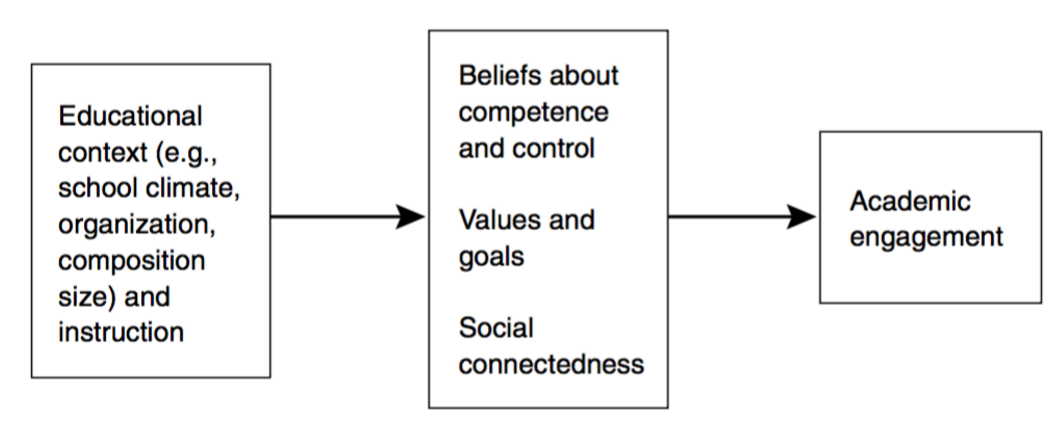
\includegraphics{../diagrams/educationalConditions.png}
\caption{A theory on educational conditions that promote intellectual
engagement}
\end{figure}

Using a blockchain as a data structure -- in this case one which is
built on a proof-of-stake consensus algorithm -- to register, manage and
save school-related educational tasks, along with a reward \& ranking
scheme linked to the blockchain, would enable students to reap immediate
rewards from their individual \& collaborative efforts. Furthermore, a
blockchain's ability to act as a pseudo-anonymous public ledger of
events, in this case school-related tasks, would provide students with
the ability to refer back to said tasks at a later point in time to
demonstrate their teamwork skills, therefore making a scarcely
confirmable skill set auditable.

\subsection{2.2 Previous Work/Existing
Applications}\label{previous-workexisting-applications}

This section gives an overview of related work within the context of
heightening student engagement described above. An observation made
while researching similar applications was that there seemed to be a
number of applications focused on digitalising and strengthening
student-to-student and student-to-teacher engagement, but none were
built in terms of a distributed, reviewable entity, such as a
blockchain.


\paragraph{SocialX}\label{socialx}

SocialX\cite{Temperini2008}\cite{Sterbini2009} is an exercise sharing tool which enables students to earn
reputation points, which are visible to their peers and the given
subject's teacher, by submitting solutions to exercises. A further
source of reputation are endorsements, which a student may receive from
their peers if they were inspired to reuse the student's solution.

\begin{figure}[htbp]
\centering
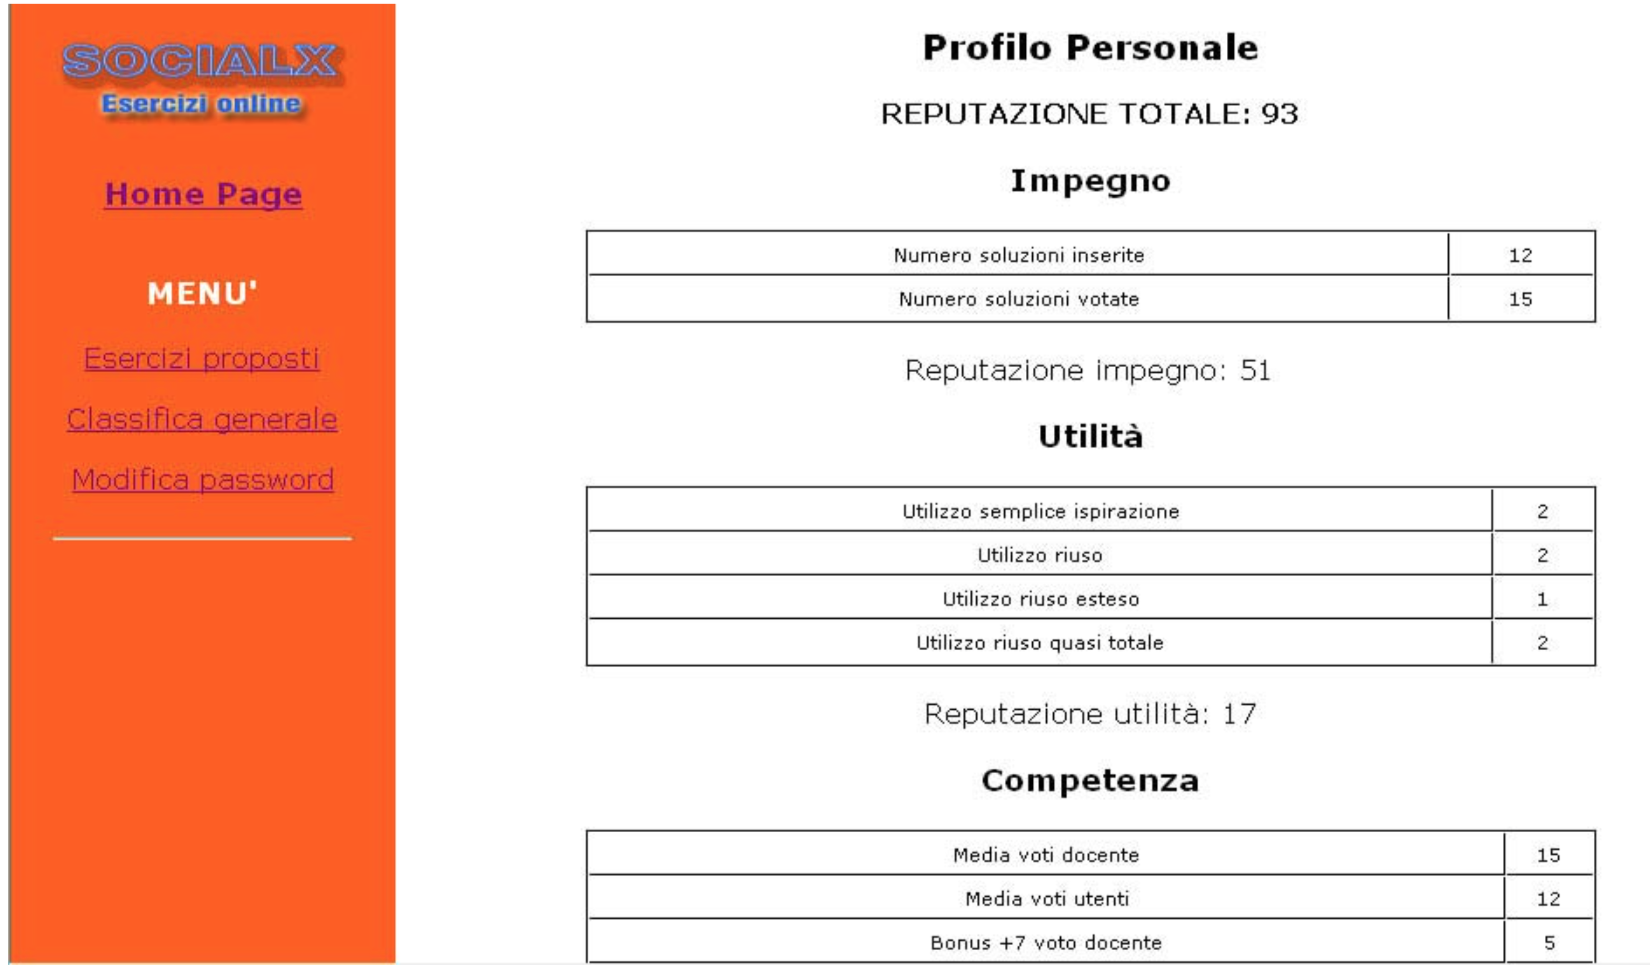
\includegraphics{../screenshots/socialx.png}
\caption{SocialX's reputation overview}
\end{figure}

SocialX differs to QuantiTeam in three key ways: firstly, reputation
within SocialX is calculated according to factors which involve the
judgment of each other's work, whereas in QuantiTeam's reputation is a
function of team size and is either rewarded in full to all team members
or not at all, depending on whether the task/exercise in question was
completed. Secondly, QuantiTeam has no teacher role, and is therefore
able to avoid a bottleneck SocialX suffers from. Thirdly, SocialX
defines the term ``global ranking'' as a measurement of student
reputation across subjects/courses, whereas QuantiTeam strives for a
truly global, decentralised ranking system.

\paragraph{WikiSpaces}\label{wikispaces}

WikiSpaces\cite{1wikispaces} is a web app which provides a virtual classroom workspace in
which teachers and students can work on written projects individually or
in teams. Features include a social media-like feed, collaborative
writing and commenting tools, and a project management system.

\begin{figure}[htbp]
\centering

\includegraphics{../screenshots/wikispaces.png}
\caption{The WikiSpaces Classroom dashboard}
\end{figure}

\paragraph{HaikuLearning}\label{haikulearning}

HaikuLearning\cite{haikulearning}, similarly to WikiSpaces, is a web app which attempts to
emulate and enhance the classroom experience for both school teachers
and students. It offer a unified environment to hand in assignments and
to receive feedback \& grades, as well as enabling integrations with
Google Apps for extensibility.

A notion which provides a key separation between QuantiTeam and these
services is that both WikiSpaces and HaikuLearning place the
metaphorical ball firmly in the court of teaching staff, as teachers
still decide what material is worked on and how, even providing the
ability to monitor students' progress. Within QuantiTeam, tasks are set
by team members themselves and contextual information regarding the
progress or completion of a user's tasks cannot be monitored by any
other individual.

\begin{figure}[htbp]
\centering
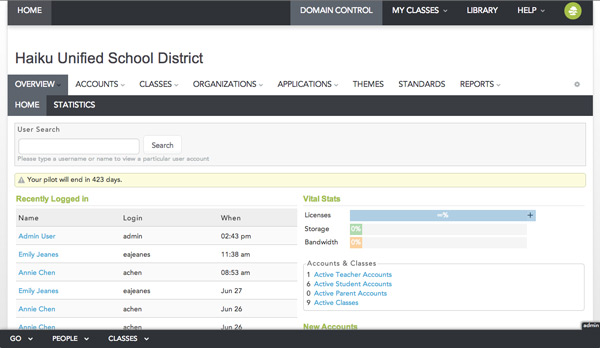
\includegraphics{../screenshots/haikulearning.jpg}
\caption{The HaikuLearning dashboard}
\end{figure}

\subsection{2.3 Programming Languages and
Libraries}\label{programming-languages-and-libraries}

\subsubsection{2.3.1 Blockchain}\label{blockchain}

Before proceeding with the following section, two frequently used
concepts should be clearly delineated: blockchains and smart contracts.
A blockchain is a data structure composed of a list of blocks of
transactions, where each block is linked back to the previous block in
the chain\cite{antonopoulos2014mastering}. Each block is identified by a
hash, which is stored in the block's header alongside the previous
block's hash, known as the parent block\cite{antonopoulos2014mastering}, thus providing a
traceable, reverse-chronological chain of transactions over time.\\
The concept of a smart contract was originally developed by Nick Szabo
in 1997, and is usually evoked in terms of a digital protocol which
enforces and/or verifies the performance of a contract between two or
more
parties\cite{1szabo}.

At the outset of the project, a key decision which had to be made was
the choice of blockchain implementation to be used. This decision was
critical, as discovering a major flaw in the implementation or an
incompatibility between what the implementation could provide and what
was needed, would have resulted in (at least temporary) deadlock for the
entire project.\\
The author's initial experimentation with
OpenChain\cite{1openchain}, which seemed to
offer the possibly useful ability to chain contracts to each other, was
quickly abandoned as the available documentation was insufficiently
detailed and partially ambiguous. This would have left the project open
to a lot of guesswork and thus the above mentioned risk of deadlock.\\
MultiChain\cite{1multichain}, on the other
hand, was an implementation which had well-defined documentation, but it
assumed a level of pre-existing familiarity with the API of a
blockchain, as well as providing preciously little context as to how
smart contracts could be developed for the platform in an effective
way.\\
The apparent drawbacks of the two mentioned blockchain implementations
therefore led the author to the
Eris\cite{1erisindustries} platform. Eris itself
provides a suite of tools which wrap and augment a
Tendermint\cite{1tendermint} blockchain
implementation. Eris's wealth of documentation and its well-structured
command line interface (henceforth CLI) were the deciding factors for it
becoming the blockchain implementation of choice. The documentation
provided not only step-by-step examples of how a developer could
configure and deploy a blockchain, but also provided in-depth tutorials
and examples on how to write \& deploy
Solidity\cite{1solidity}
smart contracts for the platform; highly valuable for a smart contract
novice such as the author. Furthermore, the fact that Tendermint is an
entirely separate software project meant that there was an additional
repository of documentation for this specific type of blockchain and the
computer science theory backing it.

\subsubsection{2.3.2 Server-side}\label{server-side}

Considering the author's background as a JavaScript developer, the
natural choice for a web server for the project was
NodeJS\cite{1node}. NodeJS provides a great
level of flexibility and extensibility thanks to its huge ecosystem of
open-source libraries available through its package manager,
NPM\cite{1npm}, thus providing an essential
basis to help mitigate the possibly complicated technical details of
interfacing with a low-level blockchain.\\
As JavaScript is an ever-evolving language, a choice had to be made as
to whether the commonly supported
ECMAScript\cite{1ecma} 5
(ES5) specification should be used or the modern standard, ES6. ES5 was
selected to provide the maximum level of compatibility for wherever the
server is being deployed, as native support for ES6 is not widespread as
of the point of writing and transpiling the server's code from ES6 to
ES5 for each deployment would have been a lot more trouble than use for
a humble web server.

QuantiTeam's server makes use of a handful of key libraries:

\paragraph{Express}\label{express}

Express\cite{1express} is a minimalist
framework for NodeJS web servers which provides a powerful layer of
abstraction on top of NodeJS's raw server interface. Express helped
accelerate the development of the API, while leaving the possibility of
fine-tuning the NodeJS server itself intact.

\paragraph{eris-wrapper \& eris-logger}\label{eris-wrapper-eris-logger}

The eris-wrapper \& eris-logger modules were adopted from a ``Hello
World''-style example Eris provides to showcase how a NodeJS server
implementing their platform could be
structured\cite{1helloeris}.\\
eris-wrapper provides a convenient abstraction of low-level bindings
that have to take place between the NodeJS server and the Tendermint
blockchain, while eris-logger simply sets up a simple logger with
different logging types, such as \texttt{ERROR}, \texttt{INFO} and
\texttt{DEBUG}.

\paragraph{Async}\label{async}

Async\cite{1async} is a utility
library that helps manage the flow of asynchronous functions, which are
a common occurrence in NodeJS. Within the scope of the server, Async was
primarily used to chain together multiple sequential interactions with
the blockchain.

\subsubsection{2.3.3 Client-side}\label{client-side}

The platform chosen for the client-side representation of the system was
that of a mobile application. While building a web application would
have been just as feasible in conjunction with the system's API, mobile
development was chosen as the preferred paradigm in order to maximise
the potential for the project's author to gain new skills, as well as
two important usability properties:

\emph{Location independence} - Users are able to check the status of
tasks, communicate with team members and receive notifications
regardless of their current surroundings.

\emph{Familiarity} - Packaging the API's graphical representation into a
mobile app provides an already familiar UI framework which users are
accustomed to, whereas web apps often have a large degree of variance in
appearance, structure and behaviour.

During the MSc's GC02 ``App Design'' course, the author and his team had
the opportunity to build a React web application which was also required
to run as a mobile application. This was achieved by wrapping the web
app with the Apache Cordova\cite{1cordova}
mobile development framework. This experience revealed two key insights
regarding the intersection between web- and mobile-based client-side
development:\\
Firstly, that Facebook's
React\cite{1react} web development
library, in liaison with Dan Abramov's
Redux\cite{1redux} library for state management,
could be applied almost seamlessly to the context of a mobile
application. React's philosophy of thinking in terms of individual view
components, together with Redux's implementation-agnostic approach to
managing the application's state, largely abstracted away the conceptual
differences between building an HTML document and building a mobile app
view.\\
Secondly, that porting a web app to a mobile app simply does not provide
an authentic native experience on a mobile device, as it is almost
impossible to account for and implement all the differences and
individual nuances in, for example, animation styles between mobile
operating systems. This resulted in the look \& feel of the application
being closer to that of a mobile browser rather than a native mobile
app.

Based on these two lessons learnt, the author decided to use Facebook's
React Native\cite{2react-native} for the project, which grafts a truly native mobile development
framework on top of the outstanding React library, along with the now
familiar Redux library.\\
React Native offers all the benefits of React (high levels of modularity
\& encapsulation, composability) while allowing the developer to hook
into events and effects of the native mobile operating system. This
means that transitioning between views smoothly or sending a push
notification, for example, becomes a trivial undertaking.\\
Redux provides a well-defined interface to manage the state of the
application's data by managing all of it through a centralised
\texttt{store} object, the contents of which can be altered exclusively
by a set of actions previously defined by the developer. This provides a
level of clarity of how the application's state mutates over time that
is hard to achieve in a traditional Model-View-Controller\cite{krasner1988description}
(henceforth MVC) approach, in which many controllers have access to the
application's state simultaneously.

Further libraries which play a key role within the client-side
application are the following:

\paragraph{redux-thunk}\label{redux-thunk}

redux-thunk\cite{1thunk}
is a helper library which enables the use of asynchronous functions as
the aforementioned actions that affect the application's state. This is
essential to allow control over how and when the client application
sends data to the blockchain, and how it fetches data from the
blockchain to then integrate it into its local state.

\paragraph{redux-logger}\label{redux-logger}

redux-logger\cite{1reduxlogger}
supplements Redux itself by automatically logging actions and the state
changes they trigger to the development console. This meant a
significant amount of time could be saved during the project by avoiding
the need for a custom logger implementation, or worse yet, littering the
codebase with sporadic logging statements.

\paragraph{tcomb-form-native}\label{tcomb-form-native}

tcomb-form-native\cite{1tcombform}
provides a framework for forms and form validation in React Native. As
form validation in particular can take up an inordinate amount of
development time, this library was essential in order to keep the
project on track given the severe time constraints in relation to its
size.

\subsubsection{2.3.4 Testing}\label{testing}

Composing unit tests for each public function of the system's API was an
essential part of the development process, especially as the Tendermint
blockchain was able to report errors within its own processes to the
NodeJS server only in the most rudimentary of terms. This meant that if
no testing suite was in place, silent breakages and undefined behaviour
were likely to occur as the API grew.

The following JavaScript libraries were used to implement unit \&
integration tests on the server:

\paragraph{Mocha}\label{mocha}

Mocha\cite{1mocha} was chosen as the testing
framework for the project due to its specific aim of simplifying the
testing of asynchronous JavaScript code. This clearly applied to the
needs of the planned API which would be largely built on asynchronous
functions.

\paragraph{Chai}\label{chai}

Chai\cite{1chai} is an assertion library for both
test-driven development (TDD) and behaviour-driven development (BDD).
More specifically, Chai's TDD \texttt{assert} function was used to keep
test assertions simple and testable against an expected result.

\paragraph{Istanbul}\label{istanbul}

Istanbul\cite{1istanbul} is a
code coverage tool which was used to gain an overview of how much of the
API was currently covered by tests. This occurred via coverage reports,
which were generated after every run of the test suite.

\subsubsection{2.3.5 Databases: SQL vs NoSQL vs
Blockchain}\label{databases-sql-vs-nosql-vs-blockchain}

Using a blockchain as the pivotal data structure backing the system
evoked an interesting question: Could the entire system be built in a
way that did not, at any point, rely on a traditional database to store
data? This would automatically provide the ability to have a distributed
database, avoiding any central point of failure and thus the potential
for catastrophic data loss. Furthermore, this approach would be the
significantly more cohesive one in terms of system architecture. Adding
a further external data source to manage auxiliary data which doesn't
neatly fit into the duties of the blockchain's smart contracts would
have introduced a further agent within the planned API, thus
significantly increasing the complexity of coordinating data retrieval
and storage operations.\\
Yet, this approach could also have a significant impact on the size and
integrity of the stored data. Unlike with a typical SQL or noSQL
database, there is -- at the time of writing -- no commonly accepted
approach as to how data should be structured in terms of smart contracts
for persistent storage in a Tendermint blockchain. This meant an initial
attempt at implementing an interface to do so would possibly contain
inefficiencies and anti-patterns in terms of data relations.

After weighing up the above-mentioned points, the choice was made to go
ahead and attempt to store all data generated by the system within the
blockchain, as choosing to add a further form of database would likely
have been significantly more bug-prone and costly in terms of
development time.

\subsection{2.4 Tooling}\label{tooling}

\subsubsection{2.4.1 Requirements and Design
Tools}\label{requirements-and-design-tools}

GanttPro\cite{1ganttpro}, an online creator and
editor for Gantt charts, was used to create a timeline for the project,
while Google Docs\cite{2googledocs}
in conjunction with draw.io\cite{1drawio} were
used to capture requirements and create UML diagrams.\\
This report was originally written in markdown and transposed to the
Latex format using pandoc\cite{1pandoc}.

\subsubsection{2.4.2 Development Tools}\label{development-tools}

\paragraph{Editor}\label{editor}

In order to avoid switching between editors to get the best development
support for disparate parts of the project's code, Github's
Atom\cite{1atom} editor was chosen due to its level
of customisability and huge selection of plugins. Atom was particularly
suited for writing React Native code thanks to Facebook's
Nuclide\cite{1nuclide} plugin, which enables Atom
to approximate a richness of features typically only found in an
Integrated Development Environment (IDE), by offering an in-built
debugger, code snippets, and Facebook's own static type analyser which
is discussed below.

\paragraph{Static Type Analyser}\label{static-type-analyser}

Flowtype\cite{1flowtype}, a static type
analyser for JavaScript, is a further in-built feature of the Nuclide
plugin. Flowtype allows the developer to define a type for a variable, a
type signature for a function, and even to create custom union \&
intersection types. Flowtype then checks whether the defined type
specifications are adhered to and warns if it detects a TypeError. This
is an incredibly useful tool for a dynamically-typed language such as
JavaScript, where unintended type coercion is a common ailment.

\paragraph{Linters}\label{linters}

ESLint\cite{1eslint} was chosen as the linter for
both the React Native app and the NodeJS server, due to its support for
detecting syntactical \& stylistic errors in both regular JavaScript and
JSX, a mix of JavaScript and HTML used by Facebook for React.\\

\paragraph{Debugging}\label{debugging}

Debugging within the project was performed in three different ways due
to the variability of environments within the technology stack. For the
React Native app, Google Chrome's
DevTools\cite{1chromedevtools}
were utilised alongside the Xcode iOS
simulator\cite{1iossimulator} in order to interact with the app and receive log outputs
side-by-side in real-time.\\
For the NodeJS server, the aforementioned \texttt{eris-logger} module
was used to log API-related logging statements to the terminal.\\
At the bare-metal level, Eris provided a way of continuously logging the
activity of the Tendermint blockchain. Due to all operations
approximating those of assembly language and thus being represented in
hexadecimal, this was not useful in terms of locating bugs, but it
provided a sanity check to ensure that the chain was performing the
expected operations when instructed to do so by the NodeJS server,
excluding a possible cause if a bug was being searched for.

\paragraph{Version Control}\label{version-control}

The \texttt{git}\cite{1git} command line utility
was used to manage the codebase's development over time, in conjunction
with GitHub\cite{1github} to provide a remote
backup. For more involved \texttt{git} operations, such as merging
branches, Atlassian's
SourceTree\cite{1sourcetree}
GUI was used to avoid mistyping complex terminal commands and thus
potentially performing unwanted changes to the version history.

\paragraph{Docker \& Shell Scripts}\label{docker-shell-scripts}

Docker\cite{1docker} is a platform which
allows the creation of self-contained virtual environments for software
development, to mitigate arbitrary local differences between development
environments. It was an essential part of the development process as
Eris's tooling leverages Docker heavily to deploy blockchain
instances.\\
Bash shell scripts (\textbf{see Appendix X}) were constructed by the
author in order to automate processes such as hydrating the local
terminal environment with variables required to run the blockchain, or
booting the Docker virtual machine and the local blockchain instance.

\clearpage

\section{Chapter 3}\label{chapter-3-1}

\section{Requirements and Analysis}\label{requirements-and-analysis}

\subsection{3.1 Problem Statement}\label{problem-statement}

As outlined in chapters 1 \& 2, the key problems the project was trying
to solve the way in which students relate to their school work on an
everyday basis, as well as investigating the feasibility of a system
which uses a distributed blockchain data structure to verify and store
data about events which represent collaborative work.\\
The conceptual diagram below shows how the basic components and
interactions within this system might look.

\begin{figure}[htbp]
\centering
\includegraphics{../diagrams/conceptDiagram.png}
\caption{An early conceptual diagram demonstrating possible interactions
with the system}
\end{figure}

\subsection{3.2 Requirements}\label{requirements}

The act of establishing requirements was entirely focused around the
question: ``What functionality does the system require, at a minimum, to
fulfill its stated aims?''. This provided a clear focus on what was
absolutely needed for a minimum viable product (henceforth
MVP)\cite{ries2009minimum} that an individual and/or group of individuals could use in
a meaningful way. This meant both functional and non-functional
requirements were focused around three domains: tasks, users, and teams.
The requirements were prioritised according to the MoSCoW
system\cite{1moscow},
with requirements being ranked from ``Must Have'' through ``Should
Have'' and ``Could Have'', with the final category being ``Won't Have
(in this development cycle)''. The project's ``Must Have'' requirements
had to be strictly limited to what was viable within the project's
timeframe, as there were a large number of known unknowns (e.g.~the
Solidity language) and unknown unknowns (unforeseeable issues with the
API, blockchain or development environment). The ``Should Have'' and
``Could Have'' categories therefore largely express targets for more
sophisticated future iterations of the system.

\begin{longtable}[]{@{}llll@{}}
\toprule
\begin{minipage}[b]{0.04\columnwidth}\raggedright\strut
ID\strut
\end{minipage} & \begin{minipage}[b]{0.64\columnwidth}\raggedright\strut
Functional Requirements\strut
\end{minipage} & \begin{minipage}[b]{0.12\columnwidth}\raggedright\strut
Category\strut
\end{minipage} & \begin{minipage}[b]{0.09\columnwidth}\raggedright\strut
MoSCoW Priority\strut
\end{minipage}\tabularnewline
\midrule
\endhead
\begin{minipage}[t]{0.04\columnwidth}\raggedright\strut
FRQ1\strut
\end{minipage} & \begin{minipage}[t]{0.64\columnwidth}\raggedright\strut
Users should be able to sign up by providing simply a username, password
and, optionally, an email address\strut
\end{minipage} & \begin{minipage}[t]{0.12\columnwidth}\raggedright\strut
Account registration\strut
\end{minipage} & \begin{minipage}[t]{0.09\columnwidth}\raggedright\strut
Must\strut
\end{minipage}\tabularnewline
\begin{minipage}[t]{0.04\columnwidth}\raggedright\strut
FRQ2\strut
\end{minipage} & \begin{minipage}[t]{0.64\columnwidth}\raggedright\strut
Users should be able to login using a username and password\strut
\end{minipage} & \begin{minipage}[t]{0.12\columnwidth}\raggedright\strut
Login\strut
\end{minipage} & \begin{minipage}[t]{0.09\columnwidth}\raggedright\strut
Must\strut
\end{minipage}\tabularnewline
\begin{minipage}[t]{0.04\columnwidth}\raggedright\strut
FRQ3\strut
\end{minipage} & \begin{minipage}[t]{0.64\columnwidth}\raggedright\strut
Any team member should be able to register a task for their team on the
network, by specifying team members involved\strut
\end{minipage} & \begin{minipage}[t]{0.12\columnwidth}\raggedright\strut
Tasks\strut
\end{minipage} & \begin{minipage}[t]{0.09\columnwidth}\raggedright\strut
Must\strut
\end{minipage}\tabularnewline
\begin{minipage}[t]{0.04\columnwidth}\raggedright\strut
FRQ4\strut
\end{minipage} & \begin{minipage}[t]{0.64\columnwidth}\raggedright\strut
Any team member is able to view both outstanding and completed
tasks\strut
\end{minipage} & \begin{minipage}[t]{0.12\columnwidth}\raggedright\strut
Tasks\strut
\end{minipage} & \begin{minipage}[t]{0.09\columnwidth}\raggedright\strut
Must\strut
\end{minipage}\tabularnewline
\begin{minipage}[t]{0.04\columnwidth}\raggedright\strut
FRQ5\strut
\end{minipage} & \begin{minipage}[t]{0.64\columnwidth}\raggedright\strut
If user is not a member of a team, they should be able to start a new
team by adding other members via their usernames\strut
\end{minipage} & \begin{minipage}[t]{0.12\columnwidth}\raggedright\strut
Team\strut
\end{minipage} & \begin{minipage}[t]{0.09\columnwidth}\raggedright\strut
Must\strut
\end{minipage}\tabularnewline
\begin{minipage}[t]{0.04\columnwidth}\raggedright\strut
FRQ6\strut
\end{minipage} & \begin{minipage}[t]{0.64\columnwidth}\raggedright\strut
Upon resolution the task reward should be added to the participants'
scores automatically and immediately\strut
\end{minipage} & \begin{minipage}[t]{0.12\columnwidth}\raggedright\strut
Tasks\strut
\end{minipage} & \begin{minipage}[t]{0.09\columnwidth}\raggedright\strut
Must\strut
\end{minipage}\tabularnewline
\begin{minipage}[t]{0.04\columnwidth}\raggedright\strut
FRQ7\strut
\end{minipage} & \begin{minipage}[t]{0.64\columnwidth}\raggedright\strut
Users should be able to issue a request to join an existing team or
create a new one upon signup\strut
\end{minipage} & \begin{minipage}[t]{0.12\columnwidth}\raggedright\strut
Account registration\strut
\end{minipage} & \begin{minipage}[t]{0.09\columnwidth}\raggedright\strut
Should\strut
\end{minipage}\tabularnewline
\begin{minipage}[t]{0.04\columnwidth}\raggedright\strut
FRQ8\strut
\end{minipage} & \begin{minipage}[t]{0.64\columnwidth}\raggedright\strut
Users should receive sign up confirmation to verify email address\strut
\end{minipage} & \begin{minipage}[t]{0.12\columnwidth}\raggedright\strut
Account registration\strut
\end{minipage} & \begin{minipage}[t]{0.09\columnwidth}\raggedright\strut
Should\strut
\end{minipage}\tabularnewline
\begin{minipage}[t]{0.04\columnwidth}\raggedright\strut
FRQ9\strut
\end{minipage} & \begin{minipage}[t]{0.64\columnwidth}\raggedright\strut
Any team member should be able to opt out of a task they were entered
for if they are not in fact involved\strut
\end{minipage} & \begin{minipage}[t]{0.12\columnwidth}\raggedright\strut
Tasks\strut
\end{minipage} & \begin{minipage}[t]{0.09\columnwidth}\raggedright\strut
Should\strut
\end{minipage}\tabularnewline
\begin{minipage}[t]{0.04\columnwidth}\raggedright\strut
FRQ10\strut
\end{minipage} & \begin{minipage}[t]{0.64\columnwidth}\raggedright\strut
Each team member can see how many other members have completed a given
task without identities being revealed in the process\strut
\end{minipage} & \begin{minipage}[t]{0.12\columnwidth}\raggedright\strut
Tasks\strut
\end{minipage} & \begin{minipage}[t]{0.09\columnwidth}\raggedright\strut
Should\strut
\end{minipage}\tabularnewline
\begin{minipage}[t]{0.04\columnwidth}\raggedright\strut
FRQ11\strut
\end{minipage} & \begin{minipage}[t]{0.64\columnwidth}\raggedright\strut
Individuals should be able to provide public links to their completed
tasks and general profile\strut
\end{minipage} & \begin{minipage}[t]{0.12\columnwidth}\raggedright\strut
Tasks\strut
\end{minipage} & \begin{minipage}[t]{0.09\columnwidth}\raggedright\strut
Should\strut
\end{minipage}\tabularnewline
\begin{minipage}[t]{0.04\columnwidth}\raggedright\strut
FRQ12\strut
\end{minipage} & \begin{minipage}[t]{0.64\columnwidth}\raggedright\strut
Users should be able to see their team's current global ranking\strut
\end{minipage} & \begin{minipage}[t]{0.12\columnwidth}\raggedright\strut
Team\strut
\end{minipage} & \begin{minipage}[t]{0.09\columnwidth}\raggedright\strut
Should\strut
\end{minipage}\tabularnewline
\begin{minipage}[t]{0.04\columnwidth}\raggedright\strut
FRQ13\strut
\end{minipage} & \begin{minipage}[t]{0.64\columnwidth}\raggedright\strut
Users should be able to recover their password if they have forgotten
it\strut
\end{minipage} & \begin{minipage}[t]{0.12\columnwidth}\raggedright\strut
Login\strut
\end{minipage} & \begin{minipage}[t]{0.09\columnwidth}\raggedright\strut
Should\strut
\end{minipage}\tabularnewline
\begin{minipage}[t]{0.04\columnwidth}\raggedright\strut
FRQ14\strut
\end{minipage} & \begin{minipage}[t]{0.64\columnwidth}\raggedright\strut
Users should be able to view incomplete tasks their involved in and past
completed tasks\strut
\end{minipage} & \begin{minipage}[t]{0.12\columnwidth}\raggedright\strut
Tasks\strut
\end{minipage} & \begin{minipage}[t]{0.09\columnwidth}\raggedright\strut
Should\strut
\end{minipage}\tabularnewline
\begin{minipage}[t]{0.04\columnwidth}\raggedright\strut
FRQ15\strut
\end{minipage} & \begin{minipage}[t]{0.64\columnwidth}\raggedright\strut
Users should be able to upload attachments related to their tasks\strut
\end{minipage} & \begin{minipage}[t]{0.12\columnwidth}\raggedright\strut
Tasks\strut
\end{minipage} & \begin{minipage}[t]{0.09\columnwidth}\raggedright\strut
Should\strut
\end{minipage}\tabularnewline
\begin{minipage}[t]{0.04\columnwidth}\raggedright\strut
FRQ16\strut
\end{minipage} & \begin{minipage}[t]{0.64\columnwidth}\raggedright\strut
Tasks should automatically resolve to status ``Complete'' once all
participants have completed them\strut
\end{minipage} & \begin{minipage}[t]{0.12\columnwidth}\raggedright\strut
Tasks\strut
\end{minipage} & \begin{minipage}[t]{0.09\columnwidth}\raggedright\strut
Should\strut
\end{minipage}\tabularnewline
\begin{minipage}[t]{0.04\columnwidth}\raggedright\strut
FRQ17\strut
\end{minipage} & \begin{minipage}[t]{0.64\columnwidth}\raggedright\strut
Users should be able to edit their account details after signing up
(email address, password);\strut
\end{minipage} & \begin{minipage}[t]{0.12\columnwidth}\raggedright\strut
User\strut
\end{minipage} & \begin{minipage}[t]{0.09\columnwidth}\raggedright\strut
Should\strut
\end{minipage}\tabularnewline
\begin{minipage}[t]{0.04\columnwidth}\raggedright\strut
FRQ18\strut
\end{minipage} & \begin{minipage}[t]{0.64\columnwidth}\raggedright\strut
Users should be able to delete their account\strut
\end{minipage} & \begin{minipage}[t]{0.12\columnwidth}\raggedright\strut
Settings\strut
\end{minipage} & \begin{minipage}[t]{0.09\columnwidth}\raggedright\strut
Should\strut
\end{minipage}\tabularnewline
\begin{minipage}[t]{0.04\columnwidth}\raggedright\strut
FRQ19\strut
\end{minipage} & \begin{minipage}[t]{0.64\columnwidth}\raggedright\strut
An individual can request help for a task from other task
participants\strut
\end{minipage} & \begin{minipage}[t]{0.12\columnwidth}\raggedright\strut
Team\strut
\end{minipage} & \begin{minipage}[t]{0.09\columnwidth}\raggedright\strut
Could\strut
\end{minipage}\tabularnewline
\begin{minipage}[t]{0.04\columnwidth}\raggedright\strut
FRQ20\strut
\end{minipage} & \begin{minipage}[t]{0.64\columnwidth}\raggedright\strut
Members may offer help to the rest of the team without a specific
request being present, to speed up any potential rendez-vous\strut
\end{minipage} & \begin{minipage}[t]{0.12\columnwidth}\raggedright\strut
Team\strut
\end{minipage} & \begin{minipage}[t]{0.09\columnwidth}\raggedright\strut
Could\strut
\end{minipage}\tabularnewline
\begin{minipage}[t]{0.04\columnwidth}\raggedright\strut
FRQ21\strut
\end{minipage} & \begin{minipage}[t]{0.64\columnwidth}\raggedright\strut
Once a rendez-vous occurs, the parties involved should be able to chat
with each other\strut
\end{minipage} & \begin{minipage}[t]{0.12\columnwidth}\raggedright\strut
Team\strut
\end{minipage} & \begin{minipage}[t]{0.09\columnwidth}\raggedright\strut
Could\strut
\end{minipage}\tabularnewline
\begin{minipage}[t]{0.04\columnwidth}\raggedright\strut
FRQ22\strut
\end{minipage} & \begin{minipage}[t]{0.64\columnwidth}\raggedright\strut
Team members should be notified via a mobile alert if a help request
affects them\strut
\end{minipage} & \begin{minipage}[t]{0.12\columnwidth}\raggedright\strut
Team\strut
\end{minipage} & \begin{minipage}[t]{0.09\columnwidth}\raggedright\strut
Could\strut
\end{minipage}\tabularnewline
\begin{minipage}[t]{0.04\columnwidth}\raggedright\strut
FRQ23\strut
\end{minipage} & \begin{minipage}[t]{0.64\columnwidth}\raggedright\strut
Users could be able to upload a profile picture\strut
\end{minipage} & \begin{minipage}[t]{0.12\columnwidth}\raggedright\strut
User\strut
\end{minipage} & \begin{minipage}[t]{0.09\columnwidth}\raggedright\strut
Could\strut
\end{minipage}\tabularnewline
\begin{minipage}[t]{0.04\columnwidth}\raggedright\strut
FRQ24\strut
\end{minipage} & \begin{minipage}[t]{0.64\columnwidth}\raggedright\strut
Users should be able to mute help request and help offer
notifications\strut
\end{minipage} & \begin{minipage}[t]{0.12\columnwidth}\raggedright\strut
Settings\strut
\end{minipage} & \begin{minipage}[t]{0.09\columnwidth}\raggedright\strut
Could\strut
\end{minipage}\tabularnewline
\bottomrule
\end{longtable}

\begin{figure}[htbp]
\centering
\includegraphics{}
\caption{Functional Requirements}
\end{figure}

\begin{longtable}[]{@{}llll@{}}
\toprule
\begin{minipage}[b]{0.05\columnwidth}\raggedright\strut
ID\strut
\end{minipage} & \begin{minipage}[b]{0.63\columnwidth}\raggedright\strut
Non-Functional Requirements\strut
\end{minipage} & \begin{minipage}[b]{0.10\columnwidth}\raggedright\strut
Category\strut
\end{minipage} & \begin{minipage}[b]{0.11\columnwidth}\raggedright\strut
MoSCoW Priority\strut
\end{minipage}\tabularnewline
\midrule
\endhead
\begin{minipage}[t]{0.05\columnwidth}\raggedright\strut
NFRQ1\strut
\end{minipage} & \begin{minipage}[t]{0.63\columnwidth}\raggedright\strut
A User who is not logged in is prevented from accessing the app\strut
\end{minipage} & \begin{minipage}[t]{0.10\columnwidth}\raggedright\strut
Security\strut
\end{minipage} & \begin{minipage}[t]{0.11\columnwidth}\raggedright\strut
Must\strut
\end{minipage}\tabularnewline
\begin{minipage}[t]{0.05\columnwidth}\raggedright\strut
NFRQ2\strut
\end{minipage} & \begin{minipage}[t]{0.63\columnwidth}\raggedright\strut
The system shall store all user passwords in the blockchain in an
encrypted format\strut
\end{minipage} & \begin{minipage}[t]{0.10\columnwidth}\raggedright\strut
Security\strut
\end{minipage} & \begin{minipage}[t]{0.11\columnwidth}\raggedright\strut
Must\strut
\end{minipage}\tabularnewline
\begin{minipage}[t]{0.05\columnwidth}\raggedright\strut
NFRQ3\strut
\end{minipage} & \begin{minipage}[t]{0.63\columnwidth}\raggedright\strut
The app should provide offline sync, saving any state changes made
during a period of no-connection\strut
\end{minipage} & \begin{minipage}[t]{0.10\columnwidth}\raggedright\strut
Persistence\strut
\end{minipage} & \begin{minipage}[t]{0.11\columnwidth}\raggedright\strut
Should\strut
\end{minipage}\tabularnewline
\begin{minipage}[t]{0.05\columnwidth}\raggedright\strut
NFRQ4\strut
\end{minipage} & \begin{minipage}[t]{0.63\columnwidth}\raggedright\strut
A team member should be able to signal a task as complete within a
maximum of 1\textasciitilde{}2 UI interactions\strut
\end{minipage} & \begin{minipage}[t]{0.10\columnwidth}\raggedright\strut
Tasks\strut
\end{minipage} & \begin{minipage}[t]{0.11\columnwidth}\raggedright\strut
Should\strut
\end{minipage}\tabularnewline
\begin{minipage}[t]{0.05\columnwidth}\raggedright\strut
NFRQ5\strut
\end{minipage} & \begin{minipage}[t]{0.63\columnwidth}\raggedright\strut
The system should accomodate for at least 1,000 teams\strut
\end{minipage} & \begin{minipage}[t]{0.10\columnwidth}\raggedright\strut
Capacity\strut
\end{minipage} & \begin{minipage}[t]{0.11\columnwidth}\raggedright\strut
Should\strut
\end{minipage}\tabularnewline
\begin{minipage}[t]{0.05\columnwidth}\raggedright\strut
NFRQ6\strut
\end{minipage} & \begin{minipage}[t]{0.63\columnwidth}\raggedright\strut
The system should accomodate for at least 100,000 tasks\strut
\end{minipage} & \begin{minipage}[t]{0.10\columnwidth}\raggedright\strut
Capacity\strut
\end{minipage} & \begin{minipage}[t]{0.11\columnwidth}\raggedright\strut
Should\strut
\end{minipage}\tabularnewline
\begin{minipage}[t]{0.05\columnwidth}\raggedright\strut
NFRQ7\strut
\end{minipage} & \begin{minipage}[t]{0.63\columnwidth}\raggedright\strut
The system should log in a user within approximately 5 seconds\strut
\end{minipage} & \begin{minipage}[t]{0.10\columnwidth}\raggedright\strut
UX\strut
\end{minipage} & \begin{minipage}[t]{0.11\columnwidth}\raggedright\strut
Should\strut
\end{minipage}\tabularnewline
\begin{minipage}[t]{0.05\columnwidth}\raggedright\strut
NFRQ8\strut
\end{minipage} & \begin{minipage}[t]{0.63\columnwidth}\raggedright\strut
The system shall respond to any interaction in no more than 10
seconds\strut
\end{minipage} & \begin{minipage}[t]{0.10\columnwidth}\raggedright\strut
UX\strut
\end{minipage} & \begin{minipage}[t]{0.11\columnwidth}\raggedright\strut
Should\strut
\end{minipage}\tabularnewline
\bottomrule
\end{longtable}

\begin{figure}[htbp]
\centering
\includegraphics{}
\caption{Non-Functional Requirements}
\end{figure}

\subsection{3.3 Use Cases}\label{use-cases}

To remain realistic in regards to the allotted time for the project, use
cases were aimed at providing a full exploration of the API rather than
a rich user experience within the first iteration of the system,
therefore ensuring that the API could remain agnostic regarding any
particular client-side context.\\
Use cases for the client-side application and the API itself were
straightforward, as the only actors within the initial scope of the
system were the individual user and the user as part of a team, meaning
there was no need for elevated permissions within the API or specialised
UI interactions, as one might see with an administrative dashboard in
other applications.

Use cases were constructed in parallel with the initial UI sketches,
thus helping to visualise the flow of user-system interactions.\\
Figure 3.4 below represents an overview of the uses cases that
were constructed, while the detailed use cases can be reviewed in
\textbf{Appendix X}.

\begin{longtable}[]{@{}llll@{}}
\toprule
ID & Use Case & Primary Actor & Secondary Actor\tabularnewline
\midrule
\endhead
UC1 & Signup & User & System\tabularnewline
UC2 & Login & User & System\tabularnewline
UC3 & AddTask & User & System\tabularnewline
UC4 & ViewTasks & User & System\tabularnewline
UC5 & TaskComment & User & System\tabularnewline
UC6 & OptOutOfTask & User & System\tabularnewline
UC7 & CheckTaskCompletion & User & System\tabularnewline
UC8 & ExternalLinkToTask & User & System\tabularnewline
UC9 & CreateTeam & User & System\tabularnewline
UC10 & CheckTeamScore & User & System\tabularnewline
UC11 & RequestHelp & User & System\tabularnewline
UC12 & OfferHelp & User & System\tabularnewline
UC13 & MuteNotifications & User & System\tabularnewline
UC14 & EditAccount & User & System\tabularnewline
UC15 & SetProfilePicture & User & System\tabularnewline
UC16 & DeleteAccount & User & System\tabularnewline
UC17 & AttachTaskFile & User & System\tabularnewline
\bottomrule
\end{longtable}

\begin{figure}[htbp]
\centering
\includegraphics{}
\caption{Use Case Overview}
\end{figure}

\subsection{3.4 Sketches}\label{sketches}

To get a sense of a viable layout and structure for the client-side app,
the author used rough sketches to visualise each view that was needed to
meet the requirements. Once a convincing layout had been established for
a view, the author created a static mockup in React's JSX, which could
then be broken down into separate components and given dynamic
properties, such as data retrieval methods, at a later point.

\subsection{3.5 System Design}\label{system-design}

The design of the system's architecture started with creating a simple
deployment diagram (Figure 3.5), which provided a high-level view of
the system's required components and the roles they would play.\\
Establishing a high-level understanding of what the system required to
provide proficient communication between any client application and the
Tendermint blockchain was an essential aspect of the initial design
phase. Decoupling the system's functionality from the specific
implementation with which the system may be represented to a user was a
crucial provision to ensure maximum reusability and compatibility of the
system, therefore following the common software engineering mantra of
\emph{``program to an interface, not an implementation''}\cite{1programtointerface}.
Within the context of the web, the most appropriate form to follow this
approach was by developing a RESTful\cite{1rest} API, thus providing a
uniform interface of data endpoints, regardless of the client requesting
said data.

\begin{figure}[htbp]
\centering
\includegraphics{../diagrams/deploymentDiagram.png}
\caption{Deployment diagram showing the system's main components}
\end{figure}

\subsubsection{3.5.1 Smart Contract
Analysis}\label{smart-contract-analysis}

The role of the smart contracts played in this project -- rather than
attempting to literally track and enforce contractual obligations
between multiple parties -- was more closely related to that of typical
classes in object-oriented programming, with the
majority of the contracts either acting as
factories\cite{gamma1995design} for composite types or implementing
operations on these types as ``manager'' contracts.

\paragraph{Factory Contracts}\label{factory-contracts}

In order to define composite types, known in Solidity as
\texttt{struct}s, a contract was defined for each domain of the system
as revealed by the requirements. This meant there was a need for
\texttt{User}, \texttt{Team} and \texttt{Task} contracts.

\paragraph{Data Structure Contract}\label{data-structure-contract}

Solidity -- as a young and constantly developing language for smart
contracts -- does not currently provide a way to iterate over storage
arrays. The language's version of objects, the \texttt{mapping} type,
which approximates what is usually known as a hash map, is also
non-iterable. This meant a custom data structure contract was needed to
store, edit and retrieve collections of type contracts.

\paragraph{Manager Contracts}\label{manager-contracts}

To avoid violating the Single Responsibility
Principle\cite{martin2003agile} of object-oriented design, there was a
need for a set of contracts which would perform operations on instances
returned by the factory contracts. This meant there was a need for a
\texttt{UserManager}, \texttt{TeamManager} and \texttt{TaskManager}
contract.

\paragraph{Linker Contract}\label{linker-contract}

The previously discussed decision to encapsulate all data generated by
the system within the blockchain led to an issue of data relations
amongst the contracts: How could a new \texttt{Task} contract be linked
to the appropriate \texttt{User} contract if there was no structured way
to do so in comparison to, for example, an SQL interface? This meant
there was a need for a higher-order \texttt{Linker} contract, dedicated
to locating and linking related contracts in such a situation.

\begin{figure}[htbp]
\centering
\includegraphics{../diagrams/simplifiedContractsClassDiagram.png}
\caption{A simplified class diagram to illustrate the relationships
between Factory, Manager and Linker contracts}
\end{figure}

\paragraph{Action Events}\label{action-events}

Solidity's lack of any real logging capabilities meant there needed to
be consideration in regard to how function calls within contracts could
be observed from the outside. Solidity does, fortunately, provide an
\texttt{event} type, which opened up the possibility of triggering such
an \texttt{event} where required and listening for it server-side, where
logging the events was a trivial matter.

\subsubsection{3.5.2 Server-side Analysis}\label{server-side-analysis}

\paragraph{API Router}\label{api-router}

Once the structure of the smart contracts had been established, the
analysis of the server-side implementation quickly revealed that the
server's structure would largely mirror that of the smart contracts.
This was the case partially due to the way Eris's JavaScript library was
implemented, but largely due to the fact that this would keep the the
final API succinct and free of unnecessary cognitive load for the author
and for any future developers.\\
The server would therefore simply act as a relay and transformer for
data travelling between the client-side application and the blockchain,
acting as a \emph{de facto} middleman. In more concrete terms, this
would involve calling relevant contract methods on the blockchain when a
certain API endpoint was requested and transforming data between
hexadecimal and UTF-8, for example. This is necessary due to Solidity's
poor support for strings at the time of writing, meaning that all
strings would have to be encoded into 32-byte fields of hexadecimal,
known in Solidity as the \texttt{bytes32} type.

\paragraph{Uploader}\label{uploader}

Meeting the requirement of letting task participants attach files
related to the their tasks was trickier than anticipated, as choosing to
develop the system's client-side as a mobile application came with a key
drawback: file management. Mobile operating systems provide only limited
capabilities to edit and manage even simple text files, meaning that the
platform was suboptimal for attaching files related to a task. For
example, if the task involves writing a report, task participants may
want to attach the final report to the task in the blockchain, thus
further corroborating their participation in it.

To resolve this usability bottleneck, the author decided to utilise the
server not just as a headless API router, but also as an uploader,
composed of a single web page, to attach files to tasks present in the
blockchain. To implement the uploader effectively, two key aspects had
to be considered:

\emph{UX consistency} - From a usability perspective, the transition
between the mobile app interface and the browser-based uploader should
be as seamless as possible. To avoid disorienting the user, the uploader
was therefore kept as straightforward as possible; a single page with a
form and a submit button.

\emph{Security} - The user would have to enter a token -- issued by the
mobile app when a new task is created -- to confirm that the upload has
a legitimate task associated to it. The use of tokens therefore prevents
automated spam and enables the identification of users uploading
material which may be malicious or illegal in nature.

\subsubsection{3.5.3 Client-side Analysis}\label{client-side-analysis}

\paragraph{Abstracting view components with
React}\label{abstracting-view-components-with-react}

React takes markedly different approach to view templating compared to
the other major web development frameworks such as Google's
AngularJS\cite{1angular}. React's philosophy
focuses on breaking a view down into its constituent parts to form
reusable components. These components can then be composed in whichever
way the developer sees fit. This level of composability comes to its
full potential in React Native, as it enables the abstraction of common
UI components within a mobile app, providing ample opportunity to even
reuse said components across different platforms. The decision to
abstract a given component was therefore made according to the following
criteria, ordered by highest weighting first:

\emph{Frequency \& variability of use} - How sensible it was to abstract
a specific component into a more generic one heavily depended on the
range of use cases it could be applied to. For example, creating a
generic navigation bar component which could contain different buttons
for different views made sense, whereas creating an abstract component
for the user's profile summary did not, since it would only be used a
single time, in a single place within the app.

\emph{Cross-platform potential} - A secondary consideration was whether
the abstraction would be useful across platforms, i.e.~between iOS and
Android. For the initial iteration of QuantiTeam which would only focus
on iOS this aspect was less significant than the frequency of use, but
it played a significant role in keeping the client-side application open
to extension at a later point nonetheless.

\paragraph{Managing state with Redux}\label{managing-state-with-redux}

While considering the responsibilities that a client-side implementation
would have to fulfill to meet the established requirements, it also
became clear that even for a simple implementation there was a
considerable amount of application state that would have to be managed
by the client. Besides being the most common choice within React Native
applications, the Redux library provides a well-structured approach to
state management, derived from the philosophy behind the Elm programming
language. Redux ensures that events which mutate state are well-defined
and that they may only take place in a single direction
(unidirectionally).\\
In concrete terms, Redux achieves these orderly state mutations by
following three interdependent
principles\cite{1redux}:

\emph{Single source of truth} - All of the application's state is stored
in a single object tree known as the \texttt{store}.

\emph{State is read-only} - Actions, which are objects describing a
possible state mutation, are the only way to modify the store and are
therefore its only source of information.

\emph{Mutation through pure functions} - Reducers, a type of pure
function, are used to take the application's current state object in
conjunction with an action describing a state mutation, to return a new
state object.

Based on these 3 principles which impose the need for a \texttt{store}
object tree, actions and reducers, state mutations within Redux can be
visualised in the following manner:

\begin{figure}[htbp]
\centering
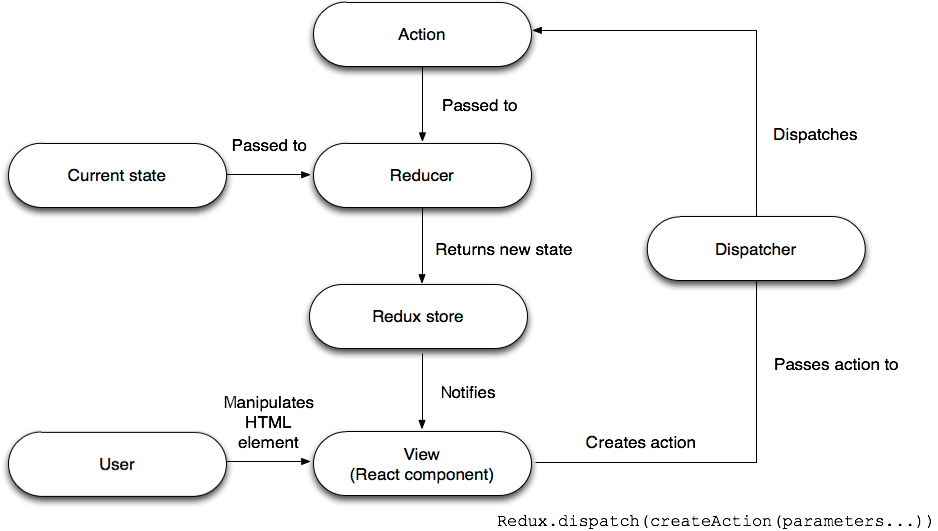
\includegraphics{../diagrams/redux.png}
\caption{State mutations within a Redux architecture\cite{1reduxibm}}
\end{figure}

\clearpage

\section{Chapter 4}\label{chapter-4-1}

\section{Design \& Implementation}\label{design-implementation}

\subsection{4.1 System Architecture}\label{system-architecture}

QuantiTeam broadly follows the three-tier architecture of a typical
Model-View-Controller\cite{krasner1988description} application with the important distinction that the
roles within the MVC pattern are applied to an entire system of various
applications, rather than a single application. In concrete terms, this
means that blockchain represents the Model element by establishing the
system's data model through the smart contracts applied to it, while the
NodeJS server represents the Controller element, providing a public
interface for client applications to issue requests to the blockchain
and handling raw responses from the blockchain. The ``View'' element of
the implementation is therefore interchangeable, as the RESTful API
formed by the web server and the blockchain provides a uniform set of
endpoints to communicate with, tying no special or unique value to the
client, in this case a mobile app.

\begin{figure}[htbp]
\centering
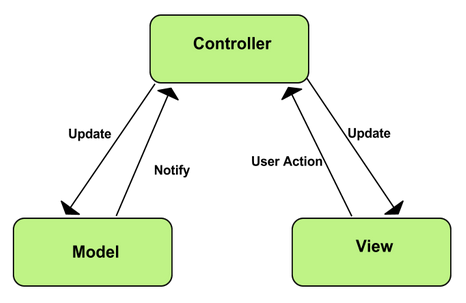
\includegraphics{../diagrams/mvc.png}
\caption{A typical MVC Model\cite{1mvcfigure}}
\end{figure}

In order to mirror the described approach of creating a standalone unit
out of the Model and Controller aspects of the system's architecture,
the project's source code was structured into two directories at the
highest level. The \texttt{app} directory contains the React Native
client-side application, while the \texttt{chain} directory holds
configurations and environment variables to run the Tendermint
blockchain via the \texttt{eris} CLI, and provides the REST API server
in its \texttt{js} subdirectory.

\subsection{4.2 Blockchain Design \&
Implementation}\label{blockchain-design-implementation}

\subsubsection{4.2.1 The Model}\label{the-model}

Within the MVC paradigm, models represent the central structure of the
application and ``are concerned with neither the user-interface nor
presentation layers but instead represent unique forms of data that an
application may
require''\cite{osmani2012learning}.\\
The Tendermint blockchain serves as a model by defining the system's
domain through the collection of smart contracts it holds, thus setting
the boundaries for what kinds of data the system is able to store and
what kind of operations can be performed on the data.

\subsubsection{4.2.2 Working with Solidity}\label{working-with-solidity}

To put a number of the design decisions made during the construction of
the blockchain's smart contracts into perspective, some context
regarding the current capabilities of the Solidity programming language
is required.

\paragraph{Strings and Numbers}\label{strings-and-numbers}

As was briefly touched upon in chapter 3, Solidity is still in its
infancy. This meant that some data types such as strings, had to be
translated into fields of 32 byte arrays in hexadecimal when fed into
the blockchain and translated vice versa when being retrieved from the
blockchain.\\
Furthermore, translating numeric values from a dynamically-typed
language such as JavaScript to a strict, statically-typed one such as
Solidity without side effects or data corruption is also no trivial
task. A point which illustrates these possibly unpredictable side
effects is the possibility of an unusually large integer being fed into
the API by a client application, which is then translated to an 8-bit
unsigned integer (\texttt{uint8}) field within a Solidity contract, thus
writing an irreparably truncated and corrupted value to the
blockchain.\\
A conscious decision was therefore made to encode all values -- aside
from booleans which are able to move across the API unaltered -- in
hexadecimal before they are fed into the blockchain, regardless of
initial type, to utilise Solidity's \texttt{bytes32} type. This approach
provided two important advantages:

\emph{Predictability} - Transforming all data associated with the
blockchain in a regular manner enhances the testability of the API by
fixing the data's representation, both when it is entered into and
retrieved from the chain. This increases the API's level testability by
making expected outputs for a given input more uniform and free of
special circumstances.

\emph{Simplicity} - Establishing a standardised format for any data to
be entered into the blockchain helped keep the API straightforward to
work with. Any numeric or string data could be encoded for the chain by
the NodeJS server using the \texttt{eris-wrapper} library module's
\texttt{str2hex()} (string-to-hex) function, and decoded using its
\texttt{hex2str()} (hex-to-string) function.

\paragraph{Arrays and Objects}\label{arrays-and-objects}

A further hindrance imposed by Solidity was its poor support for arrays
and its lack of objects, also known as lists and dictionaries,
respectively.

While JavaScript is composed entirely of objects, Solidity provides the
\texttt{mapping} type; a data structure similar to what is commonly
known as a hash map. This would have provided a sufficient
parallel to translate data formatted in JavaScript Object
Notation\cite{1json} (henceforth JSON) into a
format digestible by Solidity contracts, were it not for the fact that
Solidity's ability to store and perform operations on its mappings and
arrays is limited at best. For example, storing user profiles (i.e.
\texttt{struct}s) in a dictionary (i.e.~a \texttt{mapping}) would have
been possible, but retrieving a particular collection of dictionary
entries would have been impossible, as neither Solidity's arrays nor its
\texttt{mapping} type are iterable data structures by themselves. More
specifically, a \texttt{mapping} can only be ``probed'' for a specific
value, making it impossible to iterate over the structure and retrieve a
subset of its properties which match a given criteria. This would have
meant searching the blockchain in any non-trivial manner would have been
highly unfeasible.\\
To mitigate this functional bottleneck in Solidity, the author adopted
an implementation of a SequenceArray\cite{Shaffer2013}, which became the
\texttt{SequenceArray.sol} contract. The SequenceArray provided a
well-defined interface of methods on top of Solidity's native array and
\texttt{mapping} types, allowing the author to focus on \emph{when} and
\emph{why} data should be manipulated or searched, rather than
\emph{how} these operations are performed.

\subsubsection{4.2.3 Smart Contracts}\label{smart-contracts}

\paragraph{Data: Factory Contracts}\label{data-factory-contracts}

The blockchain's factory contracts were a straightforward undertaking,
both in regards of design and implementation, as their only role was to
return a new instance of the contract, which would then be handled by
the associated manager contracted. This meant the factory contract would
simply contain its required fields and a constructor, as shown in
\textbf{Appendix X}.

Solidity's inability to process an externally passed JavaScript object
is nicely exemplified here, due to the sheer verbosity of the
constructor function. While a task could be encapsulated as a single
object and therefore passed as a single parameter within the client- and
server-side JavaScript applications, the object had to be split into its
constituent fields by the NodeJS server before it could be handed to the
blockchain. This created what is commonly referred to as a ``code
smell''\cite{tufano2015codesmell}, by forcing the author to
implement an excessively large amount of parameters. This made both the
factory contracts themselves and the server's methods that deconstructed
the initial JavaScript object for the blockchain brittle, as any change
to a factory contract's fields had cascading effects throughout the API,
thus creating an unnecessary opportunity for bugs to appear if
refactoring was not done in a meticulous manner.

\paragraph{Operations: Manager
Contracts}\label{operations-manager-contracts}

As a contract type, Manager contracts are chiefly responsible for
indexing and modifying instances of data domain contracts, returned to
them by their respective factory contract. How a Manager-type contract
fulfills this role is exemplified with the code snippet below, which is
an extract from the \texttt{UserManager} contract's \texttt{addUser()}
method:

\begin{verbatim}
// ...
if (isOverwrite) {
    return 0x0;
} else {
    User u = new User(_id, _username, _email, _name, _password);
    userList.insert(_username, u);
    return u;
}
// ...
\end{verbatim}

The method previously checks whether the username already exists in the
\texttt{userList} sequence array and writes the result to the
\texttt{isOverwrite} variable, indicating that this would be an
``overwrite'' rather than a ``create'' operation. If the username
already exists \texttt{addUser()} returns \texttt{0x0}, a null pointer
address, thus indicating to the NodeJS server that adding the user
failed. This again exemplifies the rather primitive state of the
Solidity language at the time of writing, as the null address has to
serve as an implicit error due to the absence of an error type within
the language.\\
If \texttt{isOverwrite} is false on the other hand, the
\texttt{UserManager} contract creates a new instance of the
\texttt{User} factory contract by invoking \texttt{new\ User(...)},
returning a pointer address which indicates the position of the newly
created \texttt{User} contract in the blockchain. This address is then
inserted into \texttt{userList}, where entries are indexed by using the
passed \texttt{\_username} variable as a key, to facilitate later
retrieval.

Furthermore, the flexibility provided by the data structure contract --
in this case a sequence array -- became especially clear during the
implementation of the Manager contracts. A Manager contract could simply
instantiate a \texttt{SequenceArray.sol} contract for its own purposes
and use only the minimum amount of SequenceArray methods it required to
fulfill its functions, by creating a wrapper function around the method,
and adding additional context as required, such as logging an event:

\begin{verbatim}
contract UserManager {
    SequenceArray userList = new SequenceArray();

    // other methods...

    function isUsernameTaken(bytes32 _username) constant returns (bool) {
        registerActionEvent("IS USERNAME TAKEN");
        return userList.exists(_username);
    }
    // ...
}
\end{verbatim}

\paragraph{Relations: Linker Contract}\label{relations-linker-contract}

The Linker contract, which is best described as a utility contract, is
responsible for linking together instances of factory contracts. As one
of the blockchain's primary purposes within QuantiTeam is to act as
persistent storage layer, this type of functionality was required in
order to emulate the entity integrity provided by primary key/foreign
key relations between tables in a relational
database\cite{1primarykeyforeignkey}.\\
For example, when a user creates a new task, thus spawning a new
\texttt{Task} contract via the \texttt{TaskManager}, the system should
be able to later identify the creator of said task. A possible solution
would have been to simply let the \texttt{TaskManager} contract
establish the link itself. Although being the most obvious solution to
the issue, it would not have scaled well across the suite of
Manager-type contracts. As the author was aware that a similar need for
linkage would arise again between \texttt{Team} and \texttt{Task}
contracts, allowing each Manager-type contract to implement its own
linking mechanism was a notion which seemed to call for a layer of
abstraction. A separate \texttt{Linker} contract was therefore
established, whose sole responsibility is to create relational links
between different types of factory contract instances. To achieve this,
each new instance of a \texttt{User} or \texttt{Team} contract also
contains a \texttt{taskAddressList} sequence array. This list is used to
hold addresses (i.e.~pointers) of tasks related to this instance of a
user or team within the system. The \texttt{Linker} contract is then
responsible for adding relevant addresses to the
\texttt{taskAddressList}, an action which is performed whenever a new
task is created.\\
The following sequence diagram illustrates how the system processes a
user attempting to add a task to the blockchain, exemplifying how and
when the \texttt{Linker} contract is invoked.

\begin{figure}[htbp]
\centering
\includegraphics{../diagrams/addTaskSeqDiagram.png}
\caption{Sequence of events for an ``Add Task'' action}
\end{figure}

\begin{figure}[htbp]
\centering
\includegraphics{../diagrams/contractsClassDiagram.png}
\caption{A full Class diagram for the system's smart contracts}
\end{figure}

\subsubsection{4.2.4 Deploying Validator
Nodes}\label{deploying-validator-nodes}

\textbf{TODO: will be added upon deployment of the system this week}

\subsection{4.3 Server Design \&
Implementation}\label{server-design-implementation}

As touched upon in the server-side analysis, the REST API server's role
is first and foremost that of a data transformer and relay, forming a
bridge between the blockchain and any given client-side implementation.
The following subsections initially present how the server was designed
to adhere to principles of both the MVC and REST design patterns,
followed by an exploration how the server performs its bridging
responsibilities in concrete terms.

\subsubsection{4.3.1 The Controller}\label{the-controller}

Controllers can be regarded as an intermediary which sit between models
and views, and are typically responsible for updating the model when
changes in the view take
place\cite{osmani2012learning}. Within QuantiTeam, the server is able to fulfill
its role as a Controller component within the system's overarching MVC
architecture, by being the deciding factor concerning the logic executed
between the moment an HTTP request is received and the moment a response
issued from the API. Furthermore, the server is also responsible for
piping any changes in data in the client-side application to the
blockchain. For example, the event of a user marking a task as
``Completed'' is persisted by the server forwarding this change to the
blockchain and altering the relevant \texttt{Task} contract accordingly.

\subsubsection{4.3.2 RESTfulness}\label{restfulness}

REST, which is an acronym for Representational State Transfer, is a
commonly used web development pattern which attempts to ensure
reliability and scalability of the web service implementing
it\cite{1rest}. Within
the context of QuantiTeam, achieving RESTfulness was key for the
system's API, as this would help ensure the system's usefulness to any
context of client-side implementation, rather than specifically a mobile
paradigm.\\
This subsection therefore describes the properties of a RESTful service
and how each applies to QuantiTeam's server-side architecture.

\paragraph{Client-Server Dichotomy}\label{client-server-dichotomy}

Crucial to the creation of an implementation-agnostic REST interface is
a separation of concerns between the client and
server\cite{1rest}.
Strictly separating client and the server roles from each other provides
portability and replaceability, as the underlying implementation of
either may change without affecting the standardised form of
communication established by the REST interface.\\
Within QuantiTeam, there is a clear client-server dichotomy between the
server which is solely concerned with handling incoming requests, and
the React Native client app, which requests data from the server and
then decides how to represent said data to the user within its local
state.

\paragraph{Stateless}\label{stateless}

Statelessness is a key constraint within the REST design, which holds
that each request should contain all information required by the service
to process the request, and the service's response should contain all
the required data to fulfill said
request\cite{1rest}.\\
Applied to QuantiTeam, the REST pattern's property of statelessness not
only helped to decouple the system's architecture by avoiding the need
for managing state across different applications, it was also the most
feasible approach to enable a straightforward way of communicating with
the Tendermint blockchain, due to the previously described frequent
requirement to transform data as it travelled to and from the
blockchain. Statelessness, in this context, meant that there was no need
to worry about intermediate representations of the data being stored and
inappropriately forwarded to either the client or the blockchain at a
later point in time.

A simple example of how the server remains stateless while fulfilling
its function as an API interface is shown in the following snippet,
taken from the \texttt{server.js} module:

\begin{verbatim}
app.post('/user/taken', function (req, res) {
    var username = req.body.username;

    log.info("POST /user/taken: ", username);
    userManager.isUsernameTaken(username, function (err, isTaken) {
        _handleErr(err, res);
        res.json({isTaken: isTaken});
    });
});
\end{verbatim}

This example shows the \texttt{/user/taken} API endpoint, which is
responsible for validating the availability of usernames. When a user
tries to sign up in the client-side app, the server receives the
proposed username in the request body (the only piece of information
required for the API to fulfill the request), with which it calls the
\texttt{userManager}'s \texttt{isUsernameTaken()} method. The method
returns an \texttt{isTaken} boolean which is written to the \texttt{res}
response object, thus providing all data necessary for the client to
make a decision regarding the availability of the proposed username.

\paragraph{Cacheable}\label{cacheable}

Responses from the REST service being implicitly or explicitly declared
as cacheable or non-cacheable is a further component of a RESTful
service\cite{1rest}, as
cacheable responses provide an opportunity to to optimise the amount of
client-server communication that is needed.\\
QuantiTeam's API currently does not provide explicit cache labels in its
responses and is therefore implicitly cacheable on the client side.
While cacheability is key to scaling a developed API, investing
significant amounts of time to implement explicit cache invalidation
within QuantiTeam's first iteration was outside of the project's scope.
Implicit caching takes place within the React Native client-side app,
which retrieves and then locally retains static information such as the
user's profile data, for example.

\paragraph{Uniform Interface}\label{uniform-interface}

A uniform technical interface -- which provides a generic, high-level
method of communication across all services within a REST architecture
-- is seen as the primary constraint which distinguishes the REST
approach from other approaches to web service
architectures\cite{1rest}.\\
For QuantiTeam, this interface was constructed by using HTTP URI paths
to define API endpoints, which a client could then issue requests to.
Uniformity was further enforced by creating the following semantic
template which all of the URI paths defined for the API would follow:

\texttt{/\textless{}data-domain\textgreater{}/\textless{}optional-subdomain\textgreater{}/:\textless{}optional-parameter\textgreater{}}

This URI template declares that the first path segment is mandatory and
shall be the data domain the request is directed towards, for example
\texttt{/user} or \texttt{/tasks}.\\
The second segment may be composed of a further specification within the
data domain, such as \texttt{/profile} for \texttt{/user}, thus forming
the path \texttt{/user/profile}.\\
The third and final segment consists of an optional request parameter,
such as \texttt{:username} which may be used to pass a parameter to the
API in a HTTP GET request. Building on the previous example, we may
therefore be able to request the profile data for user \texttt{foo} by
issuing a request to the API via the path \texttt{/profile/user/foo}.

By requiring all interactions with the API to take place in this form,
the system is thus able to guarantee a high level of independence from
concrete implementation details, as the requirements and formatting of
HTTP do not vary across implementation contexts.

\paragraph{Layered System}\label{layered-system}

The final constraint within the REST pattern concerns composability. A
RESTful implementation should allow for intermediate layers, commonly
known as middleware, to be inserted into the service without affecting
the interface for communication in any
way\cite{1rest}.\\
QuantiTeam meets this constraint through its HTTP URI interface, which
enables middleware to implement the same interface and forward a given
request to the service itself using the same exact URI once it has
completed its part of processing the request.

\subsection{4.3.3 Data Handling}\label{data-handling}

An essential function of the NodeJS server is to act as data handler,
thus defining the way data has to be formatted to flow between the React
Native client app and the blockchain. As the server implements an API
interface which should be suitable for any client-side implementation,
the data transformations required took the form of translating
JavaScript objects coming from the client to a hexadecimal format in
order to adhere to Solidity's \texttt{bytes32} type, for the reasons
that were laid out in chapter 3. This was achieved by use of a
``pipeline'' function.\\
The pipeline function was defined within the utility module
\texttt{chainUtils.js} as
\texttt{marshalForChain(\textless{}data-object\textgreater{})}, which
can be reviewed in full in \textbf{Appendix X}. The function takes its
\texttt{\textless{}data-object\textgreater{}} parameter, identifies the
type of each object property (e.g.
\texttt{Array.isArray(\textless{}property\textgreater{})}) and
transforms it into a string representation of itself. Representing all
of the \texttt{\textless{}data-object\textgreater{}}s properties as
strings in an intermediate step is necessary in order to utilise the
\texttt{eris-wrapper} library module's
\texttt{str2hex(\textless{}string\textgreater{})} (string-to-hex)
function, which accepts a string as a parameter and transforms it into a
32-byte hexadecimal string. \texttt{str2hex} is therefore the final step
in the \texttt{marshalForChain} function, preparing each of the object's
properties to be fed into the blockchain.

When retrieving data from the blockchain, the transformations are
reversed via \texttt{eris-wrapper}'s \texttt{convertibleCallback()}
function, which the author modified to accept an array of transformation
functions, rather than a single function. This enables a similar
pipeline effect to that of the \texttt{marshalForChain} function, as a
property that is known to be an array can therefore be transformed back
to this representation after it has been decoded from hexadecimal to a
string via the \texttt{hex2str} (hex-to-string) function.

\texttt{contract.participants(\ eris.convertibleCallback(callback,\ {[}eris.hex2str,\ JSON.parse{]})\ )}

The snippet above shows \texttt{convertibleCallback} is invoked on a
\texttt{Task} contract's \texttt{participants} field. Aside from being
passed the \texttt{callback} parameter which will receive the
transformation's result, the function also receives an array of
transformation functions; in this case \texttt{hex2str} to decode the
hexadecimal string, followed by \texttt{JSON.parse} to convert the
string back into its original form: a JavaScript array.

\subsection{4.4 Client-side Design \&
Implementation}\label{client-side-design-implementation}

\subsubsection{4.4.1 The View}\label{the-view}

Within the MVC pattern, views are the component responsible for the
graphical representation of the application's -- or in this case the
system's -- data
models\cite{krasner1988description}.
Although a view may also be described as ``a visual representation of
models that present a filtered view of the current
state''\href{https://addyosmani.com/resources/essentialjsdesignpatterns/book/\#detailmvc}{(Learning
JS Design Patterns)}, the parallels between the MVC pattern and
QuantiTeam's structure become somewhat less applicable. While the
client-side React Native app does of course act as a filtered graphical
representation of the blockchain's models, it also contains its own
local state and therefore deviates from the typical description of an
MVC pattern's view.

\subsubsection{4.4.2 JavaScript: Emulating Strict
Typing}\label{javascript-emulating-strict-typing}

One of the key elements in designing and implementing a well-defined
client-side application for this system was the ability to define types
in a static manner and compose union and intersection types with
Facebook's Flowtype. The author found that having to think in terms of
explicit, strict type constraints made the React Native app's code more
robust and helped create better abstractions, as JavaScript's
dynamically-typed nature seemed more of a hindrance rather than a tool
when the goal was to enforce types between a client and the system's
API.\\
A pertinent example of how Flowtype helped define more robust React
components is the \texttt{Tab} type:

\begin{verbatim}
type Tab =
    'tasks'
  | 'team'
  | 'me'
  ;
\end{verbatim}

Here Flowtype allows the definition of a \texttt{Tab} enum by using
literal
types\cite{1flowtype}. The \texttt{Tab} enum was useful to specify which string
identifiers, each associated with a given view, were legal values in the
\texttt{TabsView} component, which renders the navigation bar at the
bottom of the app's viewport.

While the ability to define enums was certainly handy, Flowtype's true
usefulness is revealed when looking at one of the system's key data
types, the \texttt{User} type:

\begin{verbatim}
type User = {
    id: number;
    name: string;
    username: string;
    score: number;
    teamname?: string;
    email?: string;
    address?: string;
}
\end{verbatim}

The snippet above shows how Flowtype enabled the author to define what
type primitives a \texttt{User} object's fields should adhere to. This
significantly reduced bug frequency, both within the app and the API
itself, by catching inadvertent type coercions or possibly undefined
values before the app's runtime environment was even entered.\\
Furthermore, the \texttt{User} type exemplifies how Flowtype allows a
differentiation between mandatory (\texttt{username}) and optional
(\texttt{teamname?}) fields, adding an element of flexibility where
needed. For example, the \texttt{address?} field cannot be defined at
the time a \texttt{User}-type object is instantiated in the client-side
application, as the hexadecimal address for the User contract can only
be returned to the client once the user has been registered in the
blockchain post-instantiation.

Finally, Flowtype elevated the ability to define actions and the
expected types of their payloads in a more fine-grained manner compared
to regular JavaScript, by enabling the author to add type constraints to
variables and functions where needed.

\texttt{\{\ type:\ \textquotesingle{}FETCH\_TASKS\_SUCCESS\textquotesingle{},\ tasks:\ Array\textless{}Task\textgreater{},\ receivedAt:\ number\ \}}

The action above is triggered upon successfully fetching a user's tasks
from from the blockchain via the API. The payload includes a
\texttt{tasks} property, which is expected to be an array of
\texttt{Task} type objects, and a \texttt{receivedAt} property, which
should be a Unix timestamp and is therefore expected to be of the type
\texttt{number}.

\subsubsection{4.4.3 React: Common
Components}\label{react-common-components}

As explained in chapter 3, React's approach towards view components aims
at enabling the developer to achieve a high level of reusability and
adaptability from said components. The following section therefore shows
how the two component attributes discussed in chapter 3, namely
frequency/variability of use and cross-platform potential, were applied
to QuantiTeam's React components.

\paragraph{Frequency \& Variability of
Use}\label{frequency-variability-of-use}

A component which encapsulates both these attributes is the
\texttt{Header} component. The \texttt{Header} component creates a
generic framework for the app's header which usually contains navigation
and action buttons, such as ``Go Back'' or ``Add Task''. This means it
has to appear within almost all of the app's views, clearly meeting the
frequency of use attribute. From a variability perspective, the
\texttt{Header} component is high-level and agnostic to specific
implementation details. For example, the header's \texttt{leftItem} and
\texttt{rightItem} attributes, representing placeholders for specific
buttons, can be implemented by using a text-based or icon-based button,
as shown in (\textbf{TODO shown in appendix X}). This permits for
concrete instances of the \texttt{Header} component to apply the button
layout most suitable for a given situation. For example, a ``Settings''
button is commonly identifiable as a cog icon, whereas the ``Add Task''
action button has no commonly identifiable icon, and therefore benefits
from simply displaying text to disambiguate what action the button will
perform if tapped.

\paragraph{Cross-Platform Potential}\label{cross-platform-potential}

The flexibility of the app header's button layouts also comes into play
regarding the component's potential for reuse across differing mobile
platforms. If neither a text- nor icon-option is specified in an
instance of the \texttt{Header} component, React Native is able to
identify the current device's platform via its \texttt{Platform.OS}
variable and can thus resort to the current platform's defaults (text
buttons on iOS, icon buttons on Android). This enhanced the flexibility
and robustness of the app overall, as the header would always be able to
render its button elements, instead of simply throwing an error due to
lack of a defined layout on one platform or another. Furthermore, the
aforementioned \texttt{Platform.OS} variable provided the opportunity to
define standard behaviour for whichever platform the \texttt{Header}
component was to be rendered on, as shown here:

\begin{verbatim}
let STATUS_BAR_HEIGHT = Platform.OS === 'ios' ? 20 : 25;
let HEADER_HEIGHT = Platform.OS === 'ios' ? 44 + STATUS_BAR_HEIGHT : 56 + STATUS_BAR_HEIGHT;
\end{verbatim}

Here the header's height is automatically determined according to the
current operating system's defaults, providing a clean high-level
abstraction that avoided the need for multiple \texttt{HEADER\_HEIGHT}
definitions. Applied to only this single instance this may seems like a
trivial abstraction, but it provided the author with a useful mechanism
to avoid unnecessary code reuse and redefinition in a number of cases,
keeping the \texttt{Header} component more transparent and less verbose.

\subsubsection{4.4.4 Redux: UI and I/O}\label{redux-ui-and-io}

To apply the Redux philosophy to QuantiTeam, actions and reducers were
modularised into a schema which follows the system's data domain (users,
teams, tasks) as shown below:

\begin{verbatim}
...
├── reducers
│   ├── rootReducer.js
│   ├── tasks.js
│   ├── team.js
│   └── user.js
...
\end{verbatim}

Splitting reducers in this manner ensured that the reasoning involved in
managing the client application's state could be broken down into its
constituent parts, providing minimal cognitive load when processing data
coming from the system's API.

The client-side application's actions were broadly split along the lines
of UI-based and I/O-based interactions, representing synchronous and
asynchronous actions, respectively. During this first iteration of
QuantiTeam the author was focused on providing a useful graphical
representation of the system's API, the vast majority of actions were of
the more complex asynchronous I/O-bound type, required to interact with
the HTTP API.

\paragraph{Synchronous UI Actions}\label{synchronous-ui-actions}

UI actions within QuantiTeam are utilised to regulate animations and
transitions within the application's UI and are limited to manipulating
the application's local state only.\\
A useful example of a UI action that is frequently invoked is the
\texttt{REFRESH\_TASKLIST} action. This action is triggered when a user
pulls down on their screen to refresh their list of tasks, thus setting
the \texttt{didRefresh} boolean flag in the app's state (the
\texttt{store}) to \texttt{true}, which in turn causes a loading icon to
be shown to the user. As the \texttt{didRefresh} flag can only be reset
by the asynchronous \texttt{FETCH\_TASKS\_SUCCESS} action, indicating
that the tasks have been retrieved from the blockchain, the loading icon
is displayed until this action is triggered. This exemplifies how Redux
imbues the application's UI state with precise controls and succinct
behaviour if actions are used effectively.

\paragraph{Asynchronous I/O Actions}\label{asynchronous-io-actions}

I/O actions within QuantiTeam are structured to enable reliable
communication with the system's API. In abstract terms, any event within
the client-side application which required data from or sent data to the
blockchain, follows a pattern involving three types of Redux
actions\cite{1redux}:

\emph{Request} - A Request action is dispatched the moment the
client-side application registers an event that requires an API
interaction to be completed, indicating that either a Success or Failure
action should soon follow. Using a user signup event as an example, the
\texttt{SIGNUP\_REQUEST} action is dispatched along with the data from
the signup form filled in by the user.

\emph{Success} - If the request issued to the API succeeds and receives
a valid response, a Success action is dispatched with said response,
which is in turn handled by its associated reducer, thus incorporating
the new data into the application's state. Within a user signup event
flow, this would dispatch the \texttt{SIGNUP\_SUCCESS} action to the
\texttt{user} reducer, along with the new \texttt{User} contract's
blockchain address pointer as its payload.

\emph{Failure} - If the request issued to the API fails for any reason,
a Failure action is dispatched, which includes the error message
returned by the failed attempt to communicate with the API. In the
context of a user's signup, this scenario would dispatch the
\texttt{SIGNUP\_FAIL} action, logging the associated error the console.

By combining these three action types, the application's I/O-bound
interactions with the API follow a standardised sequence, thus providing
clear and deterministic behaviour, as the methodology of retrieving data
remains the same while the underlying data being operated upon may
change.

\section{Chapter 5}\label{chapter-5-1}

\section{Testing}\label{testing-1}

\subsection{5.1 Testing Strategy}\label{testing-strategy}

Once the required communication abilities for the system had been
established, meaning the author was able to trigger smart contract
events within the blockchain via HTTP requests, the system's API was
established and expanded via test-driven development. This meant that
any new functions of the system would be developed in the following
manner\cite{beck2003test}:

\begin{enumerate}
\def\labelenumi{\arabic{enumi}.}
\tightlist
\item
  A new test is added for the unwritten, proposed function. This ensures
  that the functions requirements are clear from the outset.
\item
  The test suite is run and the new test should fail. This excludes
  false positives (i.e.~the test always passes) and confirms that the
  functionality does not in fact exist yet.
\item
  The minimum amount of code necessary to make the new test pass is
  written.
\item
  The test suite is run again. If tests fail, adjustments are made to
  the new function until all tests pass.
\end{enumerate}

The system was therefore tested through a sequence of tests which became
increasingly high-level over time as its functionality grew; beginning
with modular unit tests, then moving onto integration tests for the API
as a whole, and concluding with functional testing from the perspective
of the client-side GUI.

\subsection{5.2 Unit Testing}\label{unit-testing}

Within QuantiTeam, unit tests are focused on providing extensive
coverage for all public API functions (known in JavaScript as ``exported
functions'') of the server's modules. As the server simply provides an
interface to the the Solidity contracts on the blockchain, this provided
a method of simultaneously testing the contracts' public functions; a
significantly more robust solution compared to attempting to construct a
reliable test suite within the Solidity language. Unit tests
purposefully excluded modules' private functions to avoid fixating the
test suite on implementation details and to avoid breaking the
encapsulation of each
module\cite{hunt2003pragmatic}. This allowed the author to focus on ensuring that the API's
components provided expected outputs to given inputs, thus implicitly
testing the functionality of private functions which are called in the
process.

The Mocha test framework -- in combination with the Chai assertion
library's \texttt{assert} function -- were used to compare a function's
returned result to an expected value:

\begin{verbatim}
describe("addTask", function () {
    it("adds the given task object to the chain and returns the registered task's hex address", function(done) {
        taskManager.addTask(testTask, function (error, address) {
            assert.isNull(error);
            assert.isString(address, "`address` should be the registered task's hex address");
            done();
        });
    });
});
\end{verbatim}

The snippet above shows the unit test for the \texttt{TaskManager}
module's public \texttt{addTask} function. Mocha's straightforward
support for asynchronous JavaScript is nicely exemplified here. The
asynchronous function's callback parameters (\texttt{error,\ address})
are checked, after which \texttt{done()} is declared, indicating to
Mocha that no further values are being awaited for this unit test.\\
API data was provided to the unit tests via mocked objects where
required, an example of which can be found in \textbf{Appendix X} for
the \texttt{TeamManager} unit tests.

\subsection{5.3 Integration Testing}\label{integration-testing}

Integration tests were implemented in a similar manner to the system's
unit tests, but were focused on providing a full examination of the
API's endpoints the system would provide and thus how differing
modules/contracts coordinate with one another. This was achieved by
encapsulating the sequence of functions required for each API endpoint
in a \texttt{chain} module with an associated \texttt{chain\_test} suite
of tests. For example, attempting to retrieve a user's tasks via the
\texttt{/tasks/:username} endpoint calls the \texttt{chain} module's
\texttt{getUserTasks} function, which in turn simply defines a sequence
of \texttt{UserManager} and \texttt{TaskManager} functions required to
fulfill the request, returning the final result. Through this
encapsulation, the author was able to define the \texttt{chain\_test}
suite of API tests which examined the API's outputs for given input
parameters, ensuring that its constituent parts integrated with one
another as expected.

\subsection{5.4 Functional Testing}\label{functional-testing}

As the blockchain and server had been tested rigorously with both unit
tests and integration tests, functional testing efforts could be focused
on examining the behaviour of the client-side app and ensuring that its
interactions with the API were represented correctly within the user
interface. Functional tests were therefore executed by running the React
Native app in the iOS simulator alongside Google Chrome's developer
console, in order to examine log output generated by Redux actions. The
\texttt{redux-logger} library showed its strength during the functional
testing stage, by letting the author easily examine the app's state
object before and after any action was triggered, thus significantly
simplifying any debugging that was required.

\subsection{5.5 Coverage}\label{coverage}

\textbf{TODO: final coverage report will be added when implementation is
complete}

\section{Chapter 6}\label{chapter-6-1}

\section{Conclusions and Project
Evaluation}\label{conclusions-and-project-evaluation}

\subsection{6.1 Project Goals}\label{project-goals-1}

At the outset of this project, the author intentionally defined the
goals at a level which would be challenging, even possibly unfeasible,
to reach in the time space available, with no other developers to split
workloads with. Considering this context, the project's goals were
largely met, forming a healthy basis for future endeavours of this kind
to build on.\\
The first and most challenging goal was to establish a functioning
public API which would allow individuals to form teams of their own
choosing and register the team's completed tasks on a blockchain. This
was achieved in what the author would classify as a ``naïve''
implementation. Section 6.4 provides details on the author's reasoning
for the term ``naïve''.\\
The second goal of the project was to build a client-side application to
showcase the API's functionality in visual terms. This goal was achieved
at a level satisfactory to the author, considering that the primary
focus of the project lay in establishing the API and the stack of
technologies backing it.\\
The third goal was to deploy a basic network of validator nodes which
would implement a true proof-of-stake consensus algorithm for the
blockchain. This was a surprisingly smooth undertaking due to the high
quality CLIs of Eris, Docker and AWS, allowing a smooth transition from
a single local node to a truly distributed set of validator nodes for
the blockchain.

\subsection{6.2 Personal Aims Achieved}\label{personal-aims-achieved}

The following section reiterates each personal aim set out by the
author, providing commentary on whether the aim has been achieved and in
what way.

\begin{itemize}
\item
  \emph{Become familiar with native mobile app development by utilising
  existing JavaScript knowledge in the context of React Native.}\\
  Using React Native to build the client-side application was as useful
  an exercise as the author had hoped it would be. Previous experience
  with React and JavaScript allowed a full focus on elements specific to
  a mobile platform, such as self-contained ListViews, which are a
  common feature in mobile development but absent in web development,
  where a list is generally an abstract concept constructed from HTML
  elements.
\item
  \emph{Learn how to write smart contracts in Solidity that are useful
  in the context of the project and for existing platforms such as
  Ethereum.}\\
  Despite initial struggles due to Solidity still being in its early
  days as a programming language, the project offered ample opportunity
  to learn how to design and implement various types of smart contracts
  and how to write idiomatic Solidity in general.
\item
  \emph{Implement a form of blockchain technology, by learning how to
  set up, run \& maintain a a blockchain proficiently.}\\
  The author feels that he was able to cover all key aspects involved in
  developing and maintaining a piece of software which leverages a form
  of blockchain technology.
\item
  \emph{Gain a fundamental understanding of Docker and how it leverages
  ``containerisation'' to achieve straightforward deployments of
  development environments.}\\
  Working with the \texttt{docker-machine} CLI to run and manage virtual
  operating system environments which could in turn run pre-packaged
  (``containerised'') software taught the author how much the usually
  arduous and fiddly task of setting up dependencies for a piece of
  software can be abstracted and simplified, by bundling the software
  along with its dependencies into a single unit, a container.
\end{itemize}

\subsection{6.3 Critical Evaluation}\label{critical-evaluation}

\subsubsection{6.3.1 Scope Feasibility}\label{scope-feasibility}

The author feels that the project's scope was challenging but
appropriate overall for the timeframe available, considering that the
project's goals were intentionally set to a high level. A realisation
which began to materialise during the final weeks of the project's
implementation stage was that it may have been more pertinent to focus
efforts entirely on the API, meaning the design and implementation of
the server and blockchain, rather than additionally providing an example
client-side implementation. While building a mobile app in React Native
was undoubtedly a useful learning experience, creating client-side
features for each feature of the API added significant time costs,
meaning a number of ``Should Have'' and ``Could Have'' requirements
which would have enhanced the API's capabilities significantly had to be
omitted due to time constraints.

\subsubsection{6.3.2 Suitability of Chosen
Technologies}\label{suitability-of-chosen-technologies}

\paragraph{Solidity Contracts \& Eris
Tooling}\label{solidity-contracts-eris-tooling}

It took the author a considerable amount of time to become accustomed
with how to write idiomatic Solidity contracts, as the programming style
required is similar to that of typical object-oriented languages, but
deviates in a number of significant ways. Despite this, Solidity's
extensive levels of documentation, along with the Eris platform's
Solidity tutorials, enabled the author to utilise the language to meet
the needs of the project.\\
The well-defined Eris CLI provided a smooth learning curve regarding how
to create, run and deploy Tendermint blockchain instances, allowing the
author to avoid significant amounts of time being wasted by the amount
of trial-and-error experimentation that would have been required to run
a Tendermint blockchain from scratch.

\paragraph{NodeJS \& Express}\label{nodejs-express}

NodeJS in combination with the Express framework, which added a powerful
level of abstraction, were the perfect choice to build the system's API
router. The author's level of familiarity with both of these
technologies, as well as JavaScript as a whole, allowed the author to
immediately mock up some functionality for the server and refactor in
confidence until a suitable production-level implementation was
established.

\paragraph{React Native, Redux \&
Flowtype}\label{react-native-redux-flowtype}

React Native was as effective as the author had hoped within the scope
of the project. Breaking views down into their constituent components
not only helped to enforce better design, it also aided in breaking down
data requirements within the client-side app, as each component is only
responsible for the data it actually requires. Prior knowledge of the
React library avoided a lengthy learning phase for the client-side
implementation, as the few concepts React Native adds are well
documented by its team at Facebook.\\
Redux was a solid choice for state management, as it ensured a level of
control and transparency out-of-the-box which is usually only achievable
through careful engineering in other libraries focused on state- and
data-management.\\
Flowtype was a powerful addition to the client-side app, allowing the
author to reason about the app's data domain in a more explicit,
type-safe manner.

\subsection{6.4 Future Work}\label{future-work}

\paragraph{Verifiability}\label{verifiability}

In Section 6.1, the author referred to the system's current
implementation as being naïve in its current state. This attribution
stems from the fact that the system currently has no means of providing
true verifiability for collaborative work in the way, for example, a
cryptographic hash may verify an entity or individual. While QuantiTeam
hashes new text files and compares them to the ones already present in
the blockchain, a coercive user simply has the ability to upload an
unrelated file and mark the associated task as completed. The system is
therefore naïve in the sense of being unaware of the possibility of
coercive agents interacting with it. QuantiTeam therefore lays the
groundwork for a system maintaining verified data on collaborative work
in a distributed manner, but has a long way to go to truly achieve this
ideal.

\paragraph{Ranking}\label{ranking}

In order to drive motivation to engage with the system on a continual
basis, providing a global ranking system in future iterations as
described in the requirements is crucial. This would significantly aid
driving a sense of achievement in task participants, as resolving a task
would immediately feed back into a virtual reward scheme. Similar to
StackOverflow's reputation
scheme\cite{1reputation}, QuantiTeam scores could become more meaningful the more
people use the system, by acting as an abstract representation of
participation in one's team to help get collaborative work done.

\paragraph{Location Data}\label{location-data}

From a perspective of extensibility, QuantiTeam could be expanded to
include geolocation data related to users and tasks, thus providing a
further possibility to corroborate the occurrence of collaborative work
between team members at a certain point in time, in a certain place.
Yet, this brings with it its own complications regarding data privacy
and security, as the ability to identify an individual's location at a
given moment in time can easily be utilised in malicious ways.

\subsection{6.5 Final Thoughts}\label{final-thoughts}

The significant challenges of this project - both anticipated and
unanticipated -- were clear to the author from the outset, making the
above assessment of QuantiTeam's shortcomings in comparison to its
requirements somewhat less painful. While the system this project has
birthed still requires significant work to fulfill its theoretical aims,
the author feels that new ground has been broken in regards to personal
programming skills and knowledge, while also hoping that this
exploration of a blockchain's capabilities in a social context will
inspire further endeavours along these lines in the future.

\printbibliography

\section{Appendix A}\label{appendix-a}

\section{Use Cases}\label{use-cases-1}

\section{Appendix B}\label{appendix-b}

\section{System Manual}\label{system-manual}

\subsection{Installation}\label{installation}

\paragraph{Dependencies}\label{dependencies}

The following dependencies are required to run a local development
instance of QuantiTeam's
\href{https://github.com/tendermint/tendermint}{Tendermint} blockchain:
- \href{https://www.docker.com/}{Docker} CLI - \texttt{docker} (\&
\texttt{docker-machine} on OSX).\\
- \href{https://erisindustries.com/}{Eris} CLI - \texttt{eris} provides
a wrapper and toolchain around the Tendermint blockchain and is used
extensively.\\
- \href{https://nodejs.org/en/}{Node.js} - v4.x upwards.\\
- \href{https://www.npmjs.com/}{NPM} - QuantiTeam relies on NPM scripts
to run tests and various other tasks.

To install the project's Node.js dependencies, ensure your present
working directory (\texttt{pwd}) is \texttt{quantiteam/chain} and run:

\begin{verbatim}
npm install
\end{verbatim}

\paragraph{Setting up}\label{setting-up}

First, let's move into QuantiTeam's API directory with the following
command:

\begin{verbatim}
cd chain
\end{verbatim}

Creating a local dev \texttt{simplechain}:\\
- Automatically: Run \texttt{simplechain.sh} in the repository's root
directory, which should start logging the chain's activities after
setup.\\
- Manually: Follow Eris's brief
\href{https://docs.erisindustries.com/tutorials/chain-making/}{tutorial}.

\subsection{Running a local development
chain}\label{running-a-local-development-chain}

Assuming we now have a functioning \texttt{simplechain} instance, let's
boot it up and configure some local environment variables. In the repo's
root directory run the following two shell scripts:

\begin{verbatim}
. ./chain-up.sh; . ./envsetup.sh
\end{verbatim}

Which should give us output similar to the following:

\begin{verbatim}
Starting "default"...
(default) Check network to re-create if needed...
(default) Waiting for an IP...
Machine "default" was started.
Waiting for SSH to be available...
Detecting the provisioner...
Started machines may have new IP addresses. You may need to re-run the `docker-machine env` command.
✓ docker-machine instance has booted
✓ eval'd local environment for docker-machine
✓ booted chain instance
CHAIN           ON     CONTAINER ID     DATA CONTAINER     IMAGE                          COMMAND     PORTS
simplechain     *      8bc5938c66       0f573eb9b3         quay.io/eris/erisdb:0.11.4     [run]       0.0.0.0:1337->1337/tcp, 0.0.0.0:46656->46656/tcp, 0.0.0.0:46657->46657/tcp

✓ booted the chain service
Running QuantiTeam environment setup...
chain_dir: /Users/<YOURNAME>/.eris/chains/simplechain
chain_dir_this: /Users/<YOURNAME>/.eris/chains/simplechain/simplechain_full_000
addr: 0D96023ED9C172AE89FF478F8C560741B6DCE5E4
'host' set to docker-machine IP: 192.168.99.100
compiler_addr:
IDI_PORT set to 8082
\end{verbatim}

We can easily verify whether the \texttt{simplechain} instance is
running as expected by following its log output:

\begin{verbatim}
npm run chainlog
\end{verbatim}

\subsection{Running the Node.js chain
service}\label{running-the-node.js-chain-service}

Now that we have a local development chain running which we can interact
with, let's spin up the chain service which will act as our API router
to interface with the local chain itself.

\paragraph{Deploying contracts}\label{deploying-contracts}

First, let's compile and deploy our Solidity smart contracts in the
\texttt{contracts} directory:

\begin{Shaded}
\begin{Highlighting}[]
\CommentTok{# `$addr` should be defined from previously running `envsetup.sh`}
\KeywordTok{npm} \NormalTok{run compile -- }\OtherTok{$addr}
\end{Highlighting}
\end{Shaded}

Anytime a change is made to the smart contracts, \texttt{compile} should
be run to deploy these changes to the running \texttt{simplechain}
instance.

\paragraph{Running tests}\label{running-tests}

Next, we'll want to run QuantiTeam's test suite to ensure everything is
working as expected:

\begin{verbatim}
npm test
\end{verbatim}

This should also provide a coverage report once all unit tests have run.

\paragraph{Booting the service}\label{booting-the-service}

The chain service itself can be built \& booted simply with:

\begin{verbatim}
npm run build
\end{verbatim}

Anytime a change is made to the node server, \texttt{build} should be
run as it builds the new service container via \texttt{docker} and
replaces it with the previous one via \texttt{eris}.\\
Please refer to \texttt{package.json} for more detailed insights into
which shell commands each NPM script executes.

\subsection{API}\label{api}

QuantiTeam's API exposes the following HTTP endpoints: - POST
\texttt{/upload} - Upload a task related file via
\texttt{multipart/form-data}.\\
- POST \texttt{/user/taken} - Check whether the the username in
\texttt{req.body.username} is already taken.\\
- POST \texttt{/user/signup} - Sign up a new user with the form data
passed in \texttt{req.body}.\\
- POST \texttt{/user/login} - Log in an existing user with the form data
passed in \texttt{req.body}.\\
- GET \texttt{/user/profile/:username} - Get the profile of the username
passed via \texttt{req.params.username}.\\
- GET \texttt{/tasks/:username} - Get the tasks of the username passed
via \texttt{req.params.username}.\\
- POST \texttt{/task} - Add a new task to the blockchain via the form
data passed in \texttt{req.body.task} for the username in
\texttt{req.body.username}.\\
- GET \texttt{/team/taken/:teamname} - Check whether the teamname passed
as \texttt{req.params.teamname} is already taken.\\
- POST \texttt{/team} - Add a new team to the blockchain via the form
data passed in \texttt{req.body.form}.\\
- GET \texttt{/team/:teamname} - Get the team profile for the teamname
passed as \texttt{req.params.teamname}.\\
- POST \texttt{/team/add-member} - Add a new member to a team with the
form data passed in \texttt{req.body.form}.

\subsection{Shutting down}\label{shutting-down}

To shut down the local chain and the \texttt{docker-machine} instance,
simply run:

\begin{verbatim}
. ./chain-down.sh
\end{verbatim}

\end{document}
